\documentclass[a4paper,11pt]{article}
%\usepackage{bibtopic}
%\usepackage{natbib}
\usepackage{pgfplotstable}
\usepackage{float}
\usepackage{amsmath}
\usepackage{amssymb}
\usepackage{fullpage}
\usepackage{rotating}
\usepackage{tikz} \usetikzlibrary{trees}
\usepackage{pbox}
\usepackage{algorithm}
\usepackage[noend]{algpseudocode}
\usepackage{listings}
\usepackage{hyperref}
\usepackage{courier}
\usepackage{graphicx}
\usepackage{epsfig}
%\usepackage{cite}
\usetikzlibrary{pgfplots.groupplots}
\usepackage{siunitx}
\sisetup{per=slash, load=abbr}

\usepackage{tikz}
% \usetikzlibrary{calc,angles,positioning,intersections}
\usepackage{pgfplots}
\pgfplotsset{width=7cm, height=10cm, compat=1.4, every axis/.append style={thick}}

\newcommand{\AnyCond}[1]{\text{Any}(#1)}
\newcommand{\BoundedCond}[1]{\text{Bounded}(#1)}
\newcommand{\Constraint}[1]{\textsc{#1}}
\newcommand{\DepProps}{\textit{DepProps}}
\newcommand{\Distinct}{\Constraint{Distinct}}
\newcommand{\Failed}{\text{Failed}}
\newcommand{\FailedCond}[1]{\text{Failed}(#1)}
\newcommand{\FixedCond}[1]{\text{Fixed}(#1)}
\newcommand{\Fixpoint}{\text{AtFixpt}}
\newcommand{\NoneCond}[1]{\text{None}(#1)}
\newcommand{\Gecode}{\textit{Gecode}}
\newcommand{\GIST}{\textit{GIST}}
\newcommand{\Propagate}{\text{Propagate}}
\newcommand{\PropConds}[1]{\text{PropConds}(#1)}
\newcommand{\Sequence}[1]{\left[#1\right]}
\newcommand{\Set}[1]{\left\{#1\right\}}
\newcommand{\Subsumed}{\text{Subsumed}}
\newcommand{\Tuple}[1]{\left\langle#1\right\rangle}
\newcommand{\Unknown}{\text{Unknown}}

\pagestyle{empty}

\renewcommand{\thesection}{\arabic{section}}
\renewcommand{\thesubsection}{\arabic{section}.\arabic{subsection}}

\title{\textbf{Implementing Tuple Variables in Gecode\\
	Bachelor Thesis \\
    Uppsala University  \\
  }
}

\author{Patrik Broman}

\date{\today}


\begin{document}
\maketitle
\interlinepenalty 10000

\begin{abstract}

In constraint programming, efficient pruning is vital to avoid unnecessary search. This thesis shows that tuple variables can be used to reduce the size of the search tree, which in turn may reduces the execution time. The tuple variables have been implemented in C++ for the Gecode library. The problem used to measure performance is finding paths through a deterministic finite automaton with transition costs.

\end{abstract}

\setcounter{tocdepth}{2}
\tableofcontents
\pagestyle{plain}

\section*{Acknowledgements}
Thanks to Jean-No\"{e}l Monette and Pierre Flener for being helpful supervisors. \\
Thanks to Joseph Scott for helping me configuring Gecode and solving a memory bug. \\
Thanks to Johan Gustafsson for helping me setting up an automatic test environment and general help with C++. \\

\section{Introduction}
Constraint programming (CP) is a declarative style programming, and is very similar to solving equations in mathematics. A problem is modelled with variables, which must satisfy certain conditions. These conditions are called \textit{constraints}. The variables are initialised with a set of possible values. Such a set is called a \textit{domain}. The main process is to remove values not satisfying the constraints from the domains until only one value is left in each domain. A state where all variables have a domain with exactly one value each is called a \textit{solution}.

When using CP, it is often a problem that it is impossible to remove invalid combinations of values from the domains. Consider a problem where we have the variables $x$ and $y$. We initialize the domains $dom(x)=\{1,2,3,4\}$ and $dom(y)=\{3,4,5,6\}$. We also use the constraint $x=y$. In this case, we can instantly remove 1 and 2 from $x$, and 5 and 6 from $y$. This leaves us with $dom(x)=\{3,4\}$ and $dom(y)=\{3,4\}$. Now, consider the same initial domains, but with the constraint $x\neq y$. We know that no solution has $x$ and $y$ such that $x=y$, but we cannot remove any value from any of the domains. 

Many CP problems could be solved more efficiently if it was possible to remove a combination of values from the variables, rather than removing the values individually. Recently, it has been shown in a paper \cite{Monette771427} that a \textit{tuple variable} can be used to link variables together. A \textit{tuple} is a mathematical object: It is an ordered list of elements. In this thesis, a \textit{tuple variable} is a variable whose domain contains tuples of integers. 

Gecode is a library for CP. Currently, Gecode supports Boolean, integer, integer set and float variables. The tuple variable type described here is an extension to the Gecode library. It is shown that it is possible to reach better performance by linking variables with tuples.

To demonstrate that tuple variables can be used to increase performance, I have implemented two different variants of tuple variables in two dimensions. One of them keeps an exact representation of the domain, while the other approximates the second dimension by just storing the boundaries. Individual boundaries are stored for each value in the first dimension. I wrote propagators for these tuple variable implementations and a reference propagator to compare performance. Because the main purpose of this thesis is to show that tuple variables can improve performance, I have intentionally avoided optimizing the code that handles the tuple variables. Even obvious and simple optimizations have been avoided. For the same reason, I have optimized the reference propagator as far as I can, and I have also asked more experienced CP-programmers for help with that.

To compare performance, I used the tuple variables to find all valid strings for a deterministic finite automaton (DFA) with costs for each transition (cDFA). A cDFA does not only tell whether a string is accepted or not, but also the total cost for that particular string. The performance is measured by studying how the execution time and size of the search tree depend on four parameters: the number of states, the size of the alphabet, the maximum cost per transition, and the size of the string. The results confirm that tuple variables can be more efficient.

\section{Background}
\subsection{Constraint Programming}
\label{sec:constraintp}
Constraint programming (CP) is a method to solve problems by modelling the problem with variables and constraints that the variables must satisfy \cite{FruehwirthMS06}. The variables have an initial domain of possible values. Then \textit{propagators} are used to remove values not satisfying the constraints. This is called \textit{pruning}. Propagators are explained in detail in Section~\ref{sec:propagators}. CP is a \textit{declarative} type of programming, which basically means that the programmer states what must hold, without stating how this is achieved. This is very much like mathematics. The \textit{constraints} work like equations.

A problem suitable for CP is a Sudoku. The most intuitive model uses a $9\times9$ matrix of integer variables. The constraints are that all variables have a domain of $\{1,\ldots,9\}$ and that all variables in a row, column, and box must be different. For a specific Sudoku, constraints are added to require certain variables to have predetermined values.

When using CP, different variable types may be used. Gecode comes with Boolean, integer, integer set, and float variable types. The available variable types limit the options to model a specific problem. With more different types available, a specific problem can be modelled in different ways. Consider the problem Eight queens\footnote{\url{https://en.wikipedia.org/wiki/Eight_queens_puzzle}}: The problem is to place 8 queens on a chess board in such a way that no queen threatens another queen. If only Boolean variables are available, the problem has to be modelled with 64 Boolean variables. With integer variables, 8 variables are sufficient. In the Boolean case, each variable $b[i][j]$ would tell whether a tile has a queen or not, while in the integer variable case each variable $x[i]$ would tell on which row the queen in column $i$ should be placed at. By analysing the Eight queens problem, it is easy to realise that a solution must have exactly one queen per column, since placing two queens at the same column would mean that they are threatening each other. 

When no propagator can prune any value, a \textit{brancher} takes over. A brancher typically splits the domain of a variable into two parts: One with an assigned value and one with the rest of the domain, thus creating a search tree. After this branching, the propagators are called again for all branches. The branchers determine the structure of the search tree. Branchers are described in Section~\ref{sec:branchers}. 

Solving a CP problem means alternating propagating and branching until some goal has been reached. The goal can, among others, be finding a solution, finding all solutions, or discovering that there are no solutions at all. The propagators have two main tasks. The most important task is to determine whether a \textit{solution} has been found or not. A \textit{solution} is a state where all variables are \textit{assigned}, which means the size of their domains are exactly one, and all propagators report that the values assigned to the variables satisfy the constraints. A state where at least one variable has been pruned to size zero is called a \textit{failure}. The second task for a propagator is pruning. A propagator does not necessarily need be able to prune, but otherwise the branchers need to do all the work. In order to reach good performance, the propagators need to prune as many values as possible. For example, if a variable $x$ has a domain of $\{1,\ldots,9\}$ and the constraint $x\le 4$ is used, a propagator could instantaneously remove the values $\{5,\ldots,9\}$ from the domain. If it does not, each value have to be tried individually.

Note that the domain of a variable never grows, and no value changes. The only thing that happens to a domain after its initialisation is that values are removed by either a propagator or a brancher. In the search tree, the variable domains in a certain node are always a subset of the variable domains of the parent node. 

\subsection{Tuple}
In a mathematical context, a tuple is a finite length sequence (ordered list) of elements. The elements can be of any type, such as numbers, sets, or functions. The elements do not need to be of the same type. An $n$-dimensional tuple is called an $n$-tuple. In this thesis, a tuple is denoted using angle brackets. For example, $\langle 3, 2, 1, 4, 2 \rangle$ is a 5-tuple. 

\subsection{Deterministic Finite Automaton}
\label{sec:dfa}
A deterministic finite automaton (DFA) is a 5-tuple: $\langle Q,\Sigma,\delta,q_0, F\rangle$, where $Q$ is a finite set of states, $\Sigma$ is called the \textit{alphabet} and is a finite set of symbols, $\delta : Q \times \Sigma \mapsto Q$  is a transition function mapping a state and a symbol to a state, $q_0\in Q$ is called the \textit{starting state}, and $F\subseteq Q$  is a set of states called \textit{accepting states} \cite{hopcroft2001introduction}. A state from which there is no path (via one or more transitions) to an accepting state is commonly called a \textit{garbage state}. Furthermore, the set of garbage states is commonly viewed as one state, called \textit{the} garbage state. Usually, the garbage state is left out in both graphical and algebraic representations. 

A DFA \textit{consumes} symbols from a string from the beginning to the end. If the DFA is in an accepting state when all symbols in the string have been consumed, then the DFA \textit{accepts} the string. Figure~\ref{fig:dfasdp} shows a 2-state DFA with omitted garbage state.

\begin{figure}[H]
\centering
\includegraphics[scale=0.6]{dfa.eps}
\caption{A DFA for the Swedish drinking protocol, as it is shown in the Gecode documentation \cite{mpg}. State $1$ is the starting state and the only accepting state. State $2$ is a non-accepting state. The symbols $d$ and $s$ denote drinking and singing. The DFA means that you may drink whenever you want, but if a song has been sung you have to drink before you leave. A regular expression for this DFA is $(d|sd)^{*}$}, but it can be expressed in different ways.
\label{fig:dfasdp}
\end{figure}

%A finite automaton where $\Sigma$ maps a state and a symbol to a set of states instead of a single state is called a nondeterministic finite automaton (NFA). Another way to define it is allowing empty string-transitions (transitions that do not consume a symbol). These transitions are denoted $\epsilon$. It is common to also allow an NFA to have multiple starting states. NFA:s and DFA:s are mathematically equivalent. Every NFA can be converted to a DFA and vice versa. The conversion from NFA to DFA is easily done with a method called \textit{powerset construction}. An NFA is typically smaller, and is often easier to construct than a corresponding DFA.

DFAs are closely related to regular expressions (regex). Every regex corresponds to a DFA and vice versa. Note that this is not true for the extended regexes one can find in many languages, such as Perl and Python. A pure regex can be written with the operators $($, $)$, $|$, and $^{*}$. One example that uses all of them is $ab(a|b)c^{*}$ which is a regex for the language of all strings starting with $ab$, continuing with either an $a$ or a $b$, and ends with zero or more $c$. A corresponding DFA for this regex is $Q=\{1,2,3,4\}, \Sigma=\{a,b,c\}, q_0=1, F=\{4\}, \delta(1,a)=2, \delta(2,b)=3, \delta(3,a)=4, \delta(3,b)=4, \delta(4,c)=4$. Any other parameter for $\delta$ returns the garbage state. One practical implication of this definition is that a pure regex can not check for matching parenthesises in a string.

In this thesis, an extended version of a DFA, a cost DFA (cDFA), is used. The difference is that the transition function not only maps a state and a symbol to a state, but to a tuple of both a state and a cost. The cost of an accepted string is equal to the sum of the costs of all transitions. Another possible approach is to define the DFA as a 6-tuple with a separate cost function. Mathematically the two approaches are equivalent. For implementation related reasons, the latter one is used in the actual code. Figure~\ref{fig:cdfasdp} shows an example of a cDFA.

In the paper Propagating Regular Counting Constraints \cite{Beldiceanu675954}, cDFA means \textit{counting DFA}. It is defined in a similar manner, and counting can be interpreted as cost. 

\begin{figure}[H]
\centering
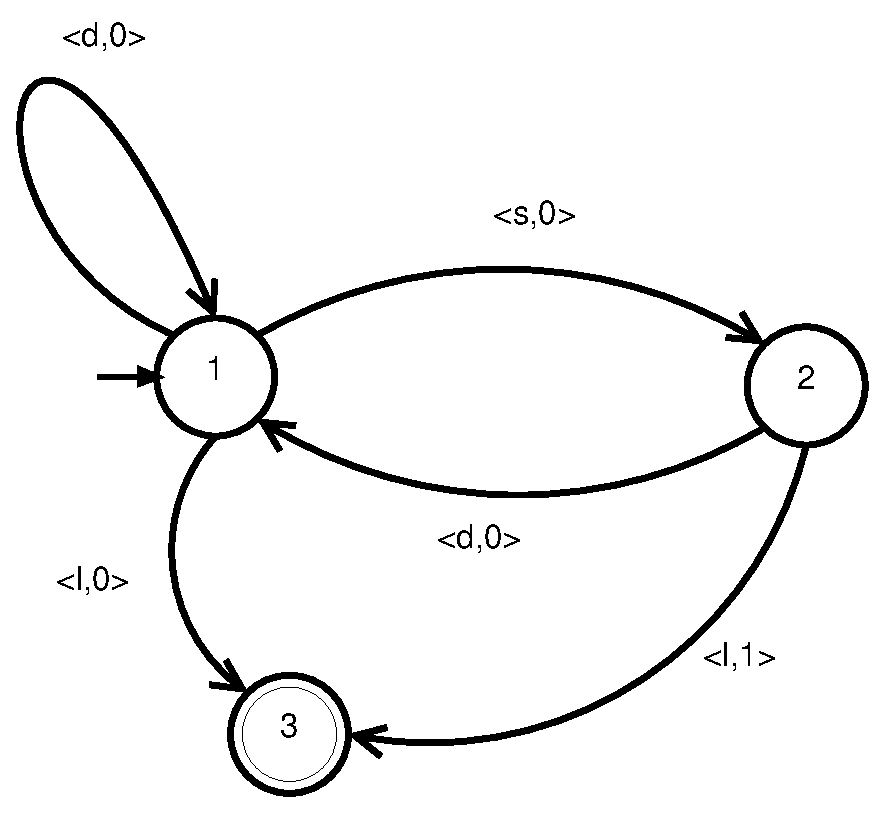
\includegraphics[scale=0.6]{cdfa.eps}
\caption{A cDFA for the Swedish drinking protocol. It is an altered variant of the DFA shown in Figure~\ref{fig:dfasdp}. The symbols $d$ and $s$ still mean drinking and singing, but the symbol $l$ is introduced for leaving. In addition, costs are introduced for all transition, so you can leave without drinking after singing, but with some added cost.}
\label{fig:cdfasdp}
\end{figure}

\subsection{The cDFA Constraint}
\label{sec:cdfaconstraint}
A \textit{constraint} is a rule that must hold for a solution. We have already looked at simple constraints, such as $x\le y$, and such. Those constraints are easy to implement, and the propagators are easy to optimise. The constraint $cDFA$ is much more complicated. It is defined such that $cDFA(state_1, cost_1, state_0, cost_0, symbol, statefun, costfun)$ holds if and only if $state_1= statefun(state_0, symbol) \land cost_1=cost_0+costfun(state_0, symbol)$. Propagators for this constraint are discussed in Section~\ref{sec:propimp}.

\subsection{Creating a Custom Variable in Gecode}
Gecode is an open source CP solver programmed in C++ and is licensed under the MIT license. It is flexible and supports customization of most parts, including variable types, branchers, and propagators. It is suitable for both education and professional use. In this thesis, Gecode 4.3.2 is used.  For more information, visit the homepage: \url{http://www.gecode.org}

The following is a summary of Chapters P, B, and V in Modeling and Programming with Gecode \cite{mpg}. 

\subsubsection{Specification File}\label{sec:specfile}
Creating the specification file is the first thing that needs to be done when designing a new variable.  A simple specification file is described in Figure~\ref{fig:minimumspecfile}.

\begin{figure}[h]
\begin{minipage}{\linewidth}
\begin{lstlisting}[frame=single]
[General]
Name:        IntTuple
Namespace:   MPG::IntTuple
[ModEvent]
Name:        FAILED=FAILED
[ModEvent]
Name:        VAL=ASSIGNED
[ModEvent]
Name:        NONE=NONE
[PropCond]
Name:        NONE=NONE
[PropCond]
Name:        VAL=ASSIGNED
ScheduledBy: VAL
[End]
\end{lstlisting}
\end{minipage}
\caption{A minimal specification file.}
\label{fig:minimumspecfile}
\end{figure}

There are three different sections in the file. The specification file must start with the [General] section and end with [End]. There are also sections for modification events and propagation conditions. The specification file is used by a configuration script to generate a base class, from which the variable implementation class will inherit.

The [General] section is simple. This is where the name and namespace of the variable are specified. Both name and namespace are arbitrary. In Gecode, the standard variables have namespace \texttt{Gecode::VarName} and, in the examples in the documentation, they instead have the namespace \texttt{MPG::VarName}.

The [ModEvent] section specifies the modification events. The modification events describe how the variables change. When a propagator wants to prune the domain of a variable, it uses the class methods that the variable implementation provides. It does not modify the domain directly. If no values are pruned, then the variable returns the modification event NONE, and if all values are pruned then it returns FAILED. When the domain of a variable gets pruned so that exactly one element remains, then ASSIGNED is returned. For all variables, modification events for NONE, FAILED, and ASSIGNED are required. More modification events may be added to avoid unnecessary executions of propagators. For example, the modification event BND can be used when only the boundaries of a domain have changed. Note that other names than the required ones are arbitrary: DOM is usually denoting when any change has been made.

The [PropCond] section describes how the propagators are scheduled, depending on how the variables have changed. For all variables, the propagation conditions for NONE and ASSIGNED are required.

\subsubsection{Variable Implementation}
The variable implementation class would, with the specification file in the previous section, be called \texttt{IntTupleVarImp} and inherit from the class \texttt{IntTupleVarBase} generated from the specification file. It has to implement a function called \texttt{assigned} that returns true iff the variable is assigned. The implementation class is the class that does all the work. This is where the modification methods are defined, and the modification methods are the only methods that directly change the domain. The implementation class implements both the getters and setters that are used by the variable class and view classes.

\subsubsection{Variable Class}
The variable class is the class that is used when modeling a problem and inherits from the variable implementation. It is a read-only interface, and a programmer that does not program any custom branchers or propagators will not use anything else than this. This class would be called \texttt{IntTupleVar} by convention.

\subsubsection{Deltas}
Deltas are used for passing information about changes to improve efficiency. In this thesis an empty class is used. The only reason it is defined at all is that some mandatory virtual functions takes deltas as arguments.

\subsubsection{Views}
The variable implementation class implements methods for modification of the variable, but the variable class does not give access to these. Instead, these are called from a view, which is a read and write interface to the implementation class.

\subsubsection{Propagators}
\label{sec:propagators}
A propagator implements constraints and prunes variables. It interacts with the views and \textit{subscribes} to variables. A propagator should subscribe to all variables it depends on. When a propagator has subscribed to a variable, it receives information whenever the domain of that variable changes in a way that is relevant. For instance, a propagator for the constraint $x\le y$ should subscribe to the maximum value of x and minimum value of y, because if none of these changes, then there is nothing the propagator can do. Subscription is done using the view classes. A propagator class must have the following methods:
\begin{itemize}
\item{post} - The method for posting a constraint, which basically is declaring that a certain constraint should be used.
\item{dispose} - This works as a destructor. The only reason Gecode does not use regular destructors is that destructors in C++ cannot take arguments.
\item{copy} - A method to copy the propagator.
\item{cost} - Estimates the cost to run the propagator. Making a good estimate does not affect the correctness, but may improve efficiency by making it easier for the Gecode engine to schedule cheap propagators before expensive ones.
\item{propagate} - The method which prunes domains and determines the status to return.
\end{itemize}
The \texttt{propagate} and \texttt{post} methods have the following possible return values:
\begin{itemize}
\item{ES\_FAILED} - There is no combination of values in the domains that satisfies the constraint. 
\item{ES\_FIX} - The propagator is at a fixpoint. It is impossible for the propagator to prune more values before a domain has changed for any of the variables the propagator has subscribed to. Further changes can be done by either a brancher or another propagator.
\item{ES\_NOFIX} - The propagator may be at a fixpoint, but it is not guaranteed. Running it once more may or may not prune some values. 
\item{ES\_SUBSUMED} - The propagator is done. Regardless of any changes made to the variables, this particular propagator will not be able to do anything more.
\end{itemize}
The propagator must be able to return ES\_FAILED and at least one of the others. ES\_NOFIX is safe to return in the sense that it does not promise anything. If it cannot be guaranteed that the propagator has reached a fixpoint, then ES\_NOFIX should be returned. 

\paragraph{Consistency}
A propagator can work with different consistencies. Bound consistency means that the propagator ensures that the bounds (min and max value for an integer variable) satisfy the constraint. Domain consistency means that all values in the whole domains are parts of at least one solution. Formally, domain consistency can be defined the following way \cite{FruehwirthMS06}: Given a constraint $C$, a value $a\in dom(x)$ for a variable $x\in vars(C)$ is said to have a \textit{support} in $C$ if there exists a tuple $t\in C$ such that $a=t[x]$ and $t[y]\in dom(y)$, for every $y\in vars(C)$. A constraint $C$ is \textit{domain consistent} if for each $x\in vars(C)$, each value $a\in dom(x)$ has a support in $C$. The notation $t\in C$ means that t is an assignment to each of the variables in $C$, satisfying the constraint. The notation $t[x]$ denotes the value assigned to variable $x$ by tuple $t$. 

Bounds consistency can be defined in a similar way. First, we define $bounds(x)$. Second, we rephrase the last sentence in the definition of domain consistency to: A constraint $C$ is \textit{bounds consistent} if for each $x\in vars(C)$, each value $a\in bounds(x)$ has a support in $C$. For an integer variable $x$, $bounds(x)$ is in general defined to $\{min(dom(x),max(dom(x)\}$. For tuple variables, we can define $bounds(t)$ to be the set of all values $v\in dom(t)$ such that $\forall v:\nexists a,b\in dom(t):v.x=a.x=b.x \land a.y \le v.y \le b.y$, but compared to the case with integers, there is no obvious definition.

If $dom(x)=\{1,5,7,8\}$ and $dom(y)=\{1,3,7\}$ and the constraint $x=y$ is applied, the propagator would yield $dom(x)=\{1,5,7\}$ and $dom(y)=\{1,3,7\}$ with bounds consistency, since there are solutions to $x=1$, $x=7$, The values $x=5$ and $y=3$ will not be not considered. If the same constraint were applied with domain consistency, then we would end up with $dom(x)=\{1,7\}$ and $dom(y)=\{1,7\}$. Pruning with domain consistency does in general cost more execution time, but results in a smaller search tree.

\subsubsection{Branchers}
\label{sec:branchers}
When there are no propagators able to prune any variable, search is performed. The branchers determine the structure of the search tree. The simplest brancher just puts the first value in the domain - according to some order - in the first branch and the rest of the values in a second branch. Another way is to pick a random value in the domain, but more sophisticated ways exist. A brancher can create an arbitrary number of nodes, but the union of all nodes must be the original domain, and at least one node must be different from the others. Ideally, the intersection between two nodes created by a brancher is empty. A brancher is not strictly needed, but if they are not used, then the propagators need to be able to prune the domains to a solution.

\subsection{Pair Variables}
When solving a problem with CP, it is desirable to minimize the search tree to avoid brute force searching. The size of the search tree depends in part on the model and the strengths of the propagators. With good models and propagators, the variable domains can be pruned to smaller sizes, keeping the branching and searching to a minimum. For example, if two variables $x$ and $y$ have domains $dom(x)=\{1,2,3\}$ and $dom(y)=\{2,3,4\}$, and the constraint $y<x$ is applied, then the domains can be pruned to $dom(x)=\{3\}$ and $dom(y)=\{2\}$ in one step, and the solution is found without searching. If we instead have the same variables and domains but instead use the constraint $x\neq y$, then nothing can be pruned, since there exist solutions for all values in both domains.

In this example, the problem was modelled with two integer variables. If the problem is modelled with one tuple variable instead of two integer variables, then pruning would be possible. In that case, we have a tuple variable $t$ with domain 
$dom(t)=\{
\langle1,2\rangle,\allowbreak 
\langle1,3\rangle,\allowbreak 
\langle1,4\rangle,\allowbreak
\langle2,2\rangle,\allowbreak
\langle2,3\rangle,\allowbreak
\langle2,4\rangle,\allowbreak
\langle3,2\rangle,\allowbreak
\langle3,3\rangle,\allowbreak
\langle3,4\rangle\}$ 
and pruning with the same constraint would yield 
$dom(t)=\{
\langle1,2\rangle,\allowbreak
\langle1,3\rangle,\allowbreak
\langle1,4\rangle,\allowbreak
\langle2,3\rangle,\allowbreak
\langle2,4\rangle,\allowbreak
\langle3,2\rangle,\allowbreak
\langle3,4\rangle\}$. 
This shrinks the size of the domain from 9 to 7. 

If we look at the case where $dom(x),dom(y)=\{1,\ldots,1000\}$ and the constraint $x=y+1$, then the benefits are more obvious. Using integer variables, only the values $x=1$ and $y=1000$ can be pruned. If tuple variables are used, then the size of the domain would shrink from $10^6$ to $10^3$. This indicates that tuple variables can be quite useful. Note though that these two examples are selected because they are easy to understand, and in reality the performance would probably drop if tuple variables were used for them. 

A more realistic example is the constraint $cDFA$ described in Section~\ref{sec:cdfaconstraint}. Furthermore, the constraint is linked in several steps: 
$cDFA(state_n, \allowbreak
cost_n,\allowbreak
state_{n-1},\allowbreak
cost_{n-1},\allowbreak
symbol_{n-1},\allowbreak
statefun, \allowbreak
costfun)$. A solution to this problem would be three arrays: one for states, one for costs, and one for symbols. With tuple variables, this could be done more efficiently by combining states and costs into one variable: 
$cDFA(P, \allowbreak
Q, \allowbreak
symbol, \allowbreak
statefun, \allowbreak
costfun)$ where $P=\langle state_1, cost_1\rangle$ and $Q=\langle state_0, cost_0\rangle$

The main benefit of a tuple variable is the possibility to link variables together. The most intuitive case is when dealing with coordinates, since a coordinate is a tuple by definition, but it can be generalized to any case where it is interesting to see if a combination of two or more values is a part of a solution. 

In general, it is more efficient to let the propagators do the work rather than the branchers. Tuple variables can move work from the branchers to the propagators. It is similar to the example with the Eight queens problem in Section~\ref{sec:constraintp}. In that case we moved work from propagators to the variables themselves.

For a pair variable $p$, the first dimension is denoted $p.x$ and the second is denoted $p.y$. For an approximate pair variable $p$, the first dimension is denoted $p.x$ and the boundaries for the second dimension is denoted $p.l$ and $p.h$ for lower and higher respectively.

\section{Implementing Pair Variables}
To keep things simple, only two-dimensional integer tuples (Pairs) are considered. Two variants are implemented. One stores an exact representation of the domain, while the other stores an overapproximation. This means that the domain is bigger than it should be. The domain still fulfills the condition that it contains all values that it should, but also some values that it should not. The approximate version only stores the boundaries for the second dimension. It stores separate boundaries for each value in the first dimension. An approximation saves memory, but the biggest benefit is that some operations can be done in constant time. A more detailed description is found in Section~\ref{sec:impapprox}. Consider the case with a tuple $t$ and the constraint $t.x\neq5$. The exact version has to remove an arbitrary amount of elements. The approximate version only needs to remove one element. 

The same benefit also holds for the following example: First we define a constraint $YLTIXEQ$ (y less than if x equal) such that $YLTIXEQ(p, a, b)$ means that $p.x=b\implies p.y<a$. With the exact variant there are possibly several values that need to be removed. The approximate version only needs to change the value of the higher bound for the element with x-value $b$.

The drawback with the approximation is that it cannot be pruned as precisely as an exact representation. This is shown in Figure~\ref{fig:pair}. However, for a cDFA problem, Beldiceanu et al. have shown that it is possible to achieve domain consistency, provided that the cost is bounded from only one direction \cite{Beldiceanu675954}.

\begin{figure}[t]
  \centering
  \pgfplotsset{  
    scale only axis,
%    xmin=1,
  }
  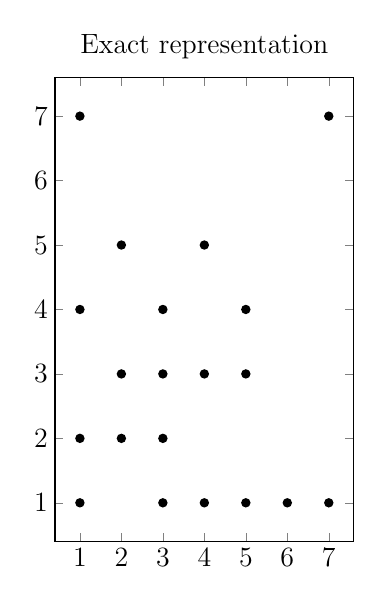
\begin{tikzpicture} [scale=0.7, font=\Large]
    \begin{axis}[
        title=Exact representation,
        xtick=data,
%        ymin=0,
      ]
      \addplot[black, mark=*, only marks]
       plot coordinates
       {  
       (1,1)       (3,1) (4,1) (5,1) (6,1) (7,1)
       (1,2) (2,2) (3,2) 
             (2,3) (3,3) (4,3) (5,3)
       (1,4)       (3,4)       (5,4)
             (2,5)        (4,5) 
       (1,7)                               (7,7)
       }; 
    \end{axis}
  \end{tikzpicture}
  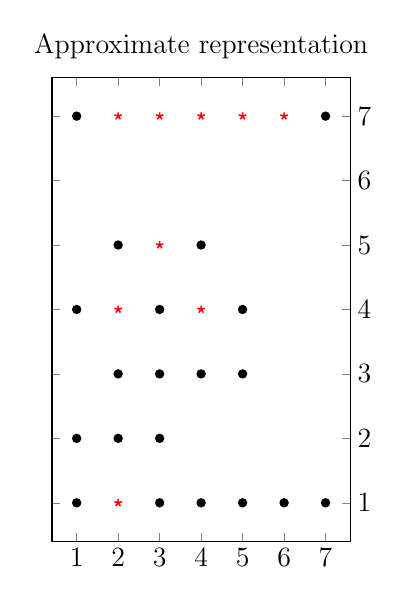
\begin{tikzpicture} [scale=0.7, font=\Large]
    \begin{axis}[
        yticklabel pos=right,
        xtick=data,
        title=Approximate representation
        ]
      \addplot[black, mark=*, only marks]
       plot coordinates
       {  
       (1,1)       (3,1) (4,1) (5,1) (6,1) (7,1)
       (1,2) (2,2) (3,2) 
             (2,3) (3,3) (4,3) (5,3)
       (1,4)       (3,4)       (5,4)
             (2,5)        (4,5) 
       (1,7)                               (7,7)
       }; 
      \addplot[red, mark=star, only marks]
       plot coordinates
       {  
             (2,1) 
       


                  (2,4)    (4,4)
                       (3,5)
            (2,7) (3,7) (4,7) (5,7) (6,7)
       }; 

    \end{axis}
  \end{tikzpicture}

 \caption{Comparison between an exact and an approximate representation of the same domain. The stars are values that should not be there, but the approximate representation only stores the boundaries for the second dimension.}\label{fig:pair}
\end{figure}


\section{Variable Design}
The specification files are kept almost as minimal as described in Section~\ref{sec:specfile}. Both implementations use identical specification files, except for the name of the variable. 

Class names follow the convention in Gecode. The variable classes are therefore named \texttt{IntPairExactVar} and \texttt{IntPairApproxVar}. 

There are three things added to the specification file described in Figure~\ref{fig:minimumspecfile}. The first two are the DOM modification event and the DOM propagating condition. These are used to schedule the propagators. As soon as the domain of any variable is changed, all propagators that have subscribed to that variable will be scheduled to run again. The last change to the specification file is the line \texttt{Dispose:true}. This is needed when using external memory resources outside Gecode. Our domains are stored as vectors from the C++ standard library, and therefore dispose is required. The way Gecode is designed, the destructors for variables are never called. If a variable needs a destructor it needs to be replaced by a method called \texttt{dispose}. This method explicitly calls \texttt{vector::$\sim$vector()}, which is the destructor for \texttt{vector}.

\begin{figure}[t]
\begin{minipage}{\linewidth}
\begin{lstlisting}[frame=single]
[General]
Name:           IntPairApprox
Namespace:      MPG::IntPairApprox
Dispose:        true
[ModEvent]
Name:           FAILED=FAILED
[ModEvent]
Name:           NONE=NONE
[ModEvent]
Name:           VAL=ASSIGNED
Combine:        VAL=VAL
[ModEvent]
Name:           DOM=SUBSCRIBE
Combine:        VAL=VAL, DOM=DOM
[PropCond]
Name:           NONE=NONE
[PropCond]
Name:           VAL=ASSIGNED
ScheduledBy:    VAL
[PropCond]
Name:           DOM
ScheduledBy:    VAL, DOM
\end{lstlisting}
\end{minipage}
\caption{The specification file for \texttt{IntPairApproxVar}. The specification file for \texttt{IntPairExactVar} is equal, except for the name and the namespace.}
\end{figure}

The main purpose of this thesis is to show that pair variables have benefits over regular integer variables for certain problems. For that reason the code for pair variables has purposely been kept unoptimised. For example, the methods implemented in the variable implementation do not use the fact that the domains are sorted. Just fixing this would decrease the time complexity from linear to logarithmic for operations like removing a value from a domain. This would be especially efficient when removing ranges of values. Currently, they are removed one by one.

The complete source can be found at \url{http://www.github.com/klutt/gecode-tuples}

\subsection{Implementation of Pair with Exact Domain}
The exact version does not approximate the domain, that is, the implementation is a long list of all integer pairs that are currently in the domain. The domain is stored as \texttt{std::vector<struct \{int x, int y\}>}. 

\paragraph{Modification Methods}
\begin{itemize}
\item {\textbf{nq(Pair p) - }} Remove the pair p from the domain. The time complexity is $\mathcal{O}(n)$, where $n$ is the number of elements in the domain.
\end{itemize}

\paragraph{Other methods}
\begin{itemize}
\item {\textbf{contains(Pair p) - }} Returns true if the domain contains the pair p, and false otherwise. The time complexity is  $\mathcal{O}(n)$, where $n$ is the number of values in the domain.
\end{itemize}

\subsection{Implementation of Pair Variables with Approximate Domain}
\label{sec:impapprox}
This version approximates the domain by just storing one dimension exactly. For the other dimension, only the boundaries are stored. Unique boundaries are stored for each value in the first dimension. The domain is stored as \texttt{std::vector<struct\{int x, int y\_low, int y\_high\}>}

\paragraph{Modification Methods}
\begin{itemize}
\item {\textbf{nq(Pair p) - }} Remove the pair p from the domain. The time complexity is $\mathcal{O}(n)$ where $n$ is the number of different x-values in domain.

\item{\textbf{yeqforspecificx(PairInterval p) - }} Remove all pairs from the domain whose y-value is not in the interval $[p.ylow; p.yhigh]$ iff those values x-values is equal to $x$. The time complexity is $\mathcal{O}(n)$, where $n$ is the number of different x-values in domain. In the actual source code the name \texttt{xeq} is used, which may be misleading. The definition of this modification method was altered during development, but the name was never changed.

\item{\textbf{xeq(PairVector v) - }} Remove all values from domain whose x-value does not exist in $v$. The time complexity is $\mathcal{O}(nm)$, where $n$ is the number of x-values in domain and $m$ is number of elements in $v$.
\end{itemize}

\paragraph{Other methods}
\begin{itemize}
\item {\textbf{contains(Pair p) - }} Returns true if the domain contains p, and false otherwise. The time complexity is $\mathcal{O}(n)$, where $n$ is number of different x-values in the domain.
\end{itemize}

\subsection{Implementation of Propagators for Constraint cDFA}
\label{sec:propimp}
The cDFA \textit{propagators} are the actual implementations of the cDFA \textit{constraint}. These propagators are implemented in three different ways. Two propagators are for pair variables and one is for integer variables. The latter one is only for reference when comparing performance. The algorithms for the propagators are described below in pseudo code.

All three implementations work in a similar manner. $PreState$ and $PreCost$ are domains containing the current state and accumulated cost so far in the cDFA. $PostState$ and $PostCost$ are the result of reading the symbol in $Symbol$. Since pair variables make it possible to bundle cost and state into a single variable, they are just called $Pre$ and $Post$. The basic principle is the following: For all symbols and all states in $Pre$, calculate the possible values for $Post$. Remove everything from $Post$ that is not reachable from any element in $Pre$. If nothing is reachable from a certain $Pre$, then also remove that element from $Pre$. This is done by creating lists containing all elements that should remain in the domains, and then removing everything from the domains that is not in those lists.

%Int
%\begin{figure}[H]
\begin{algorithm}[H]
\label{fig:algint}
\caption{DFA propagator IntVar\newline
 $\mathcal{O}(\#(PostState)\#(PostCost)\#(PreState)\#(PreCost)\#(Symbol))$ in time}
\begin{algorithmic}[1]
\Procedure{DFAprop}{IntVar PostState, IntVar PostCost, IntVar PreState, IntVar PreCost, IntVar Symbol, Statefunction S, Costfunction C}
\State Intdomain newPostState, newPreState, newPostCost, newPreCost, newSymbol := $\emptyset$
\ForAll {symbol in Symbol}
	\ForAll {preState \textbf{in} PreState}
		\State \textbf{int} state := S(pre.state, symbol)
		\If {PostState.contain(state) \textbf{and} p.state $\neq$ garbage state}
					\State newPostState := newPostState $\cup$ state
			\State newPreState := newPreState $\cup$ pre
			\State newSymbol := newSymbol $\cup$ symbol 
			\ForAll {cost \textbf{in} PreCost}
				\State int postCost := cost + C(preState, symbol)
				\If {PostCost.contains(postCost)}
					\State newPreCost := newPreCost $\cup$ cost
					\State newPostCost := newPostCost $\cup$ postCost
				\EndIf
			\EndFor
		\EndIf
	\EndFor
\EndFor
\State PostState := PostState $\cap$ newPostState
\State PreState := PreState $\cap$ newPreState
\State PostCost := PostCost $\cap$ newPostCost
\State PreCost := PreCost $\cap$ newPreCost
\State Symbol := Symbol $\cap$ newSymbol
\EndProcedure
\end{algorithmic}
\end{algorithm} 
%\caption{Propagator for DFA constraint for IntVar variables}\label{fig:algint}
%\end{figure}

%Exact
%\begin{figure}[H]
\begin{algorithm}[H]
\begin{algorithmic}[1]
\Procedure{DFAprop}{IntPairVar Post, IntPairVar Pre, IntVar Symbol, Statefunction S, Costfunction C}
\State Pairdomain newPost, newPre := $\emptyset$
\State Intdomain newSymbol := $\emptyset$
\ForAll {symbol \textbf{in} Symbol}
	\ForAll {pre \textbf{in} Pre}
		\State Pairdomain p := (S(pre.state, symbol), pre.cost+C(pre.state, symbol))
		\If {Post.contain(p) \textbf{and} p.state $\neq$ garbage state}
			\State newPost := newPost $\cup$ p
			\State newPre := newPre $\cup$ pre
			\State newSymbol := newSymbol $\cup$ symbol 
		\EndIf
	\EndFor
\EndFor
\State Post := Post $\cap$ newPost
\State Pre := Pre $\cap$ newPre
\State Symbol := Symbol $\cap$ newSymbol
\EndProcedure
\end{algorithmic}
\caption{DFA propagator IntPairExact \newline
 $\mathcal{O}(\#(Post)\#(Pre)\#(Symbol))$ in time}
\label{fig:algexact}
\end{algorithm}
%\caption{Propagator for DFA constraint for IntPairExactVar variables}\label{fig:algexact}
%\end{figure}
%Approx
%\begin{figure}[H]
\begin{algorithm}[H]
\label{fig:algapprox}
\caption{DFA propagator IntPairApprox\newline $\mathcal{O}(\#(Post)\#(Pre)\#(Symbol))$ in time}
\begin{algorithmic}[1]
\Procedure{Merge}{Pairdomain dom, Pair p}
	\State find d in dom such that d.state = p.state
	\If{not found} 
		\State add p to dom
	\Else	
		\State d.u := max(d.u, p.u)
		\State d.l := min(d.l, p.l)
	\EndIf
\EndProcedure
\Procedure{DFAprop}{IntPairVar Post, IntPairVar Pre, IntVar Symbol, Statefunction S, Costfunction C}
\State Pairdomain newPost, newPre := $\emptyset$
\State Intdomain newSymbol := $\emptyset$
\ForAll {s \textbf{in} Symbol}
	\ForAll {pre \textbf{in} Pre}
		\State tc:= C(pre.state, s)
		\State Pairdomain p :=(S(pre.state,s),pre.l+tc,pre.u+tc)
		\State i := getIndex(Post, p.x) \textit{\# Returns -1 if not found}
		\State Pairdomain q :=(S(pre.state,s),max(pre.l,P[i].l), min(pre.u,P[i].u))
		\If {p.state $\neq$ garbage state \textbf{and} q.l$\leq$q.u \textbf{and} i$\geq$0}
			\State Merge(newPost, p)
			\State Merge(newPre, q)
			\State newSymbol := newSymbol $\cup$ s
		\EndIf
	\EndFor
\EndFor
\State Post := Post $\cap$ newPost
\State Pre := Pre $\cap$ newPre
\State Symbol := Symbol $\cap$ newSymbol
\EndProcedure
\end{algorithmic}
\end{algorithm}
%\caption{Propagator for DFA constraint for IntPairApprox variables}\label{fig:algapprox}
%\end{figure}

The differences between the algorithms are adjustments to make the algorithms work with different variable types. For approximate integer variables, we can not freely remove any value we want. That is why it has the function \textsc{Merge}, which checks if there is an element $d$ in the domain $dom$ such that $d.x=p.x$. If so, then $d.y\_low$ and $d.y\_high$ get expanded to fit the interval $p.y\_low$ to $p.y\_high$. 

The \texttt{contain} functions' time complexity is $\mathcal{O}(n)$, where $n$ is the size of the domain for the Pair variables. It is fairly safe to assume that this is faster for the integer variables on average. The time complexity for the intersection operations is at most quadratic, but it does not matter since they are performed outside the loop. The union operation inside the loop is constant in time.

At a first glance it may seem that the \texttt{IntPairExactVar} propagator has better time complexity. This is an illusion, because the size of $\#(Pre)$ and $\#(Post)$ is equal to $\#(PreState)\#(PreCost)$ and $\#(PostState)\#(PostCost)$ respectively. However, this is not the case for the IntPairApproxVar propagator. Here $\#(Pre)=\#(PreState)$ and $\#(Post)=\#(PostState)$. 

The propagator for IntPairExactVar achieves domain consistency. The propagator for IntPairApproxVar does not, but this would be impossible because the domain is only approximated.

\section{Results}
In this section it is explained how the correctness of the code was verified, and how the performance was measured and compared.

\subsection{Correctness Verification}
The correctness is verified in several steps. For all problems, an \texttt{assert} is used to ensure that the solution printed actually is a valid solution before it is printed. This ensures that no false solutions occur. There are a number of trivial tests in \texttt{testsrc/} with pre-calculated numbers of solutions. If the numbers of solutions are correct, all solutions are unique, and all solutions fullfill the requirements, then we know that the code works correctly for the particular data used in the test.

For bigger problems, it is very hard to pre-calculate the number of solutions. Instead, the tests rely on probability. The two pair variants and the integer variant are compared to ensure that they put out the same number of solutions, and that the solutions are the same. It is unlikely that they would be wrong in the exact same way. These tests are found in \texttt{tripletestsrc/} and \texttt{multisteptestsrc/}.

\subsection{Performance Test}
\label{sec:performancetest}
To test the performance, the same problem is solved in three different ways. Two of them are the exact and approximate pair variables. The last one is solved with the integer variable that comes with Gecode, and is for reference. The problem is finding all the strings of a fixed length accepted by a cDFA with one accepting state. Branching is done on the symbols only, since this is enough. Indeed, if the cDFA is in a state $s$ and has a current cost $c$ and the symbol $x$ is read, then the next state and cost can be uniquely calculated. The executables accept six arguments: 

\begin{itemize}
\item{seed} - The seed for the random generator to generate the same DFA for all executables.
\item{states} - Number of states.
\item{symbols} - Size of the alphabet.
\item{cost} - Maximum cost per transition in the cDFA. This is decreased by one, so setting this to 1 means no cost.
\item{max cost} - Maximum cumulative cost for the string.
\item{steps} - Length of the string.
\end{itemize}
The test is performed by varying one parameter among $states$, $symbols$, $cost$ and $steps$, while keeping the others fixed. For each method and combination of parameters ten random cDFA are generated. All three methods generate the same cDFA for a given seed. Runtime and number of nodes are the total for the random generated DFA. The maximum total cost is set to $(steps\cdot cost)/5$. The minimum total cost for the final stage is set to the maximum total cost for each state, subtracted by 2. Below, the graphs are shown. There are four graphs for the case where the length of the string is varied: two linear and two logarithmic. The other three only have linear graphs. The graphs show number of nodes and runtime.

\begin{figure}[H]
  \centering
  \pgfplotsset{
	    scaled y ticks=false,
    scale only axis,
    legend style={at={(0,0.8)}, anchor=west , font=\tiny
    },
    xmin=7,
  }
  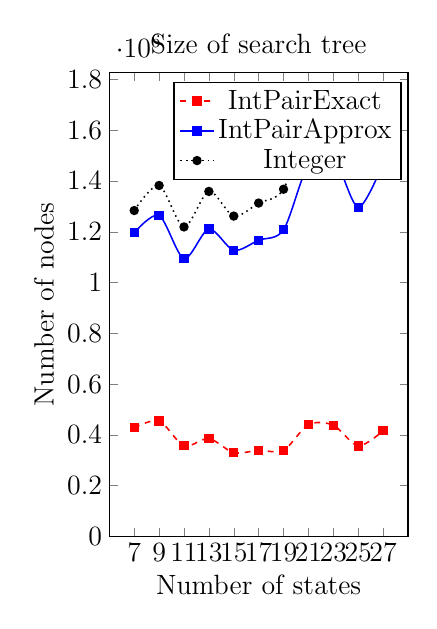
\begin{tikzpicture} [scale=0.7, font=\Large]
    \begin{axis}[
        title=Size of search tree,
        ylabel=Number of nodes,
        xtick=data,
        ymin=0, 
%        yticklabel style={/pgf/number format/sci},
%        yticklabel={ 
%        \pgfmathfloatparsenumber{\tick} 
%        \pgfmathfloatexp{\pgfmathresult} 
%        \pgfmathprintnumber{\pgfmathresult} 
%        },
        xlabel=Number of states ]
      \addplot[smooth,mark=square*, mark options={solid},red, dashed]
      coordinates{ (7,427514) (9,454874) (11,356896) (13,385169) (15,329868) (17,338722) (19,339050) (21,440084) (23,437965) (25,356520) (27,415702)
      }; %\label{ie_plot}
      \addlegendentry{IntPairExact}
      \addplot[smooth,mark=square*, mark options={solid},blue]
      coordinates{ (7,1195984) (9,1264044) (11,1094910) (13,1210487) (15,1127178) (17,1166840) (19,1207856) (21,1464930) (23,1496955) (25,1296590) (27,1470000)
      }; %\label{ia_plot}
      \addlegendentry{IntPairApprox}
      \addplot[smooth,mark=*,mark options={solid},black, dotted]
      coordinates{ (7,1283617) (9,1382304) (11,1219058) (13,1358874) (15,1261790) (17,1313042) (19,1367570) (21,1636624) (23,1661830) (25,1464554) (27,1653812)
      }; %\label{int_plot}
      \addlegendentry{Integer}
    \end{axis}
  \end{tikzpicture}
  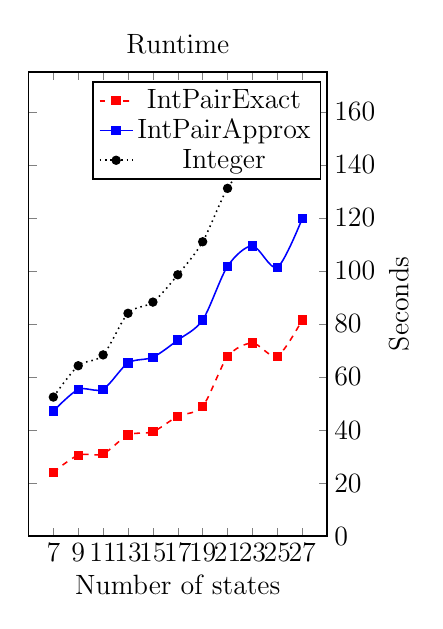
\begin{tikzpicture} [scale=0.7, font=\Large]
    \begin{axis}[
        yticklabel pos=right,
        xtick=data,
        title=Runtime,
        ylabel=Seconds,
        xlabel=Number of states,
        ymin=0, ]
      \addplot[smooth,mark=square*,mark options={solid},red, dashed]
      coordinates{ (7, 24.091) (9, 30.492) (11, 31.026) (13, 38.125) (15, 39.380) (17, 45.187) (19, 48.943) (21, 67.630) (23, 72.791) (25, 67.855) (27, 81.536)
      };% \label{IntPairExact Run}
      \addplot[smooth,mark=square*,mark options={solid},blue]
      coordinates{ (7, 47.133) (9, 55.287) (11, 55.408) (13, 65.274) (15, 67.460) (17, 73.920) (19, 81.508) (21, 101.759) (23, 109.442) (25, 101.353) (27, 119.748)
      }; %\label{IntPairApprox Run}
      \addplot[smooth,mark=*,mark options={solid},black, dotted]
      coordinates{ (7, 52.426) (9, 64.242) (11, 68.331) (13, 84.028) (15, 88.250) (17, 98.554) (19, 111.021) (21, 131.160) (23, 141.472) (25, 137.661) (27, 159.120)
      }; %\label{IntegerRun}
      \addlegendentry{IntPairExact}
      \addlegendentry{IntPairApprox}
      \addlegendentry{Integer}
    \end{axis}
  \end{tikzpicture}

%  \begin{tikzpicture}[scale=1.4]
%    \draw[very thick] (-4,0) -- (4,0);
%    \draw[draw=white] (-5,-0.2) -- (5,-0.2);
%  \end{tikzpicture}


%  \begin{tikzpicture} [scale=0.8]
%    \begin{semilogyaxis}[
%        title=No nodes logarithmic scale,
%        ylabel=nodes,
%        xtick=data,
%        ymin=0, 
%        xlabel=states ]
%     \addplot[smooth,mark=square*, mark options={solid},red, dashed]
%      coordinates{ (7,427514) (9,454874) (11,356896) (13,385169) (15,329868) (17,338722) (19,339050) (21,440084) (23,437965) (25,356520) (27,415702)
%      }; %\label{ie_plot}
%      \addlegendentry{IntPairExact}
%      \addplot[smooth,mark=square*, mark options={solid},blue]
%      coordinates{ (7,1195984) (9,1264044) (11,1094910) (13,1210487) (15,1127178) (17,1166840) (19,1207856) (21,1464930) (23,1496955) (25,1296590) (27,1470000)
%      }; %\label{ia_plot}
%      \addlegendentry{IntPairApprox}
%      \addplot[smooth,mark=*,mark options={solid},black, dotted]
%      coordinates{ (7,1283617) (9,1382304) (11,1219058) (13,1358874) (15,1261790) (17,1313042) (19,1367570) (21,1636624) (23,1661830) (25,1464554) (27,1653812)
%      }; %\label{int_plot}
%      \addlegendentry{Integer}

%    \end{semilogyaxis}
%  \end{tikzpicture}
%  \begin{tikzpicture} [scale=0.8]
%    \begin{semilogyaxis}[
%        title=Runtime logaritmhic scale,
%        yticklabel pos=right,
%        xtick=data,
%        ylabel=runtime (ms),
%        xlabel=states,
%        ymin=0,  ]
%      \addplot[smooth,mark=square*,mark options={solid},red, dashed]
%      coordinates{ (7, 24091) (9, 30492) (11, 31026) (13, 38125) (15, 39380) (17, 45187) (19, 48943) (21, 67630) (23, 72791) (25, 67855) (27, 81536)
%      }; %\label{IntPairExact Run}
%      \addplot[smooth,mark=square*,mark options={solid},blue]
%      coordinates{ (7, 47133) (9, 55287) (11, 55408) (13, 65274) (15, 67460) (17, 73920) (19, 81508) (21, 101759) (23, 109442) (25, 101353) (27, 119748)
%     }; %\label{IntPairApprox Run}
%      \addplot[smooth,mark=*,mark options={solid},black, dotted]
%      coordinates{ (7, 52426) (9, 64242) (11, 68331) (13, 84028) (15, 88250) (17, 98554) (19, 111021) (21, 131160) (23, 141472) (25, 137661) (27, 159120)
%      }; %\label{IntegerRun}
%      \addlegendentry{IntPairExact}
%      \addlegendentry{IntPairApprox}
%      \addlegendentry{Integer}
%    \end{semilogyaxis}
%  \end{tikzpicture}
 \caption{Varying the number of states. The other parameters are fixed. Size of alphabet=7, max cost per transition=15, and number of steps=7.}\label{fig:states}
\end{figure}

\begin{figure}[H]
  \centering
  \textbf{Varying symbols }
  \newline
  \newline
  \pgfplotsset{
    scale only axis,
    legend style={at={(0,0.8)}, anchor=west, font=\tiny},
    xmin=7,
  }
  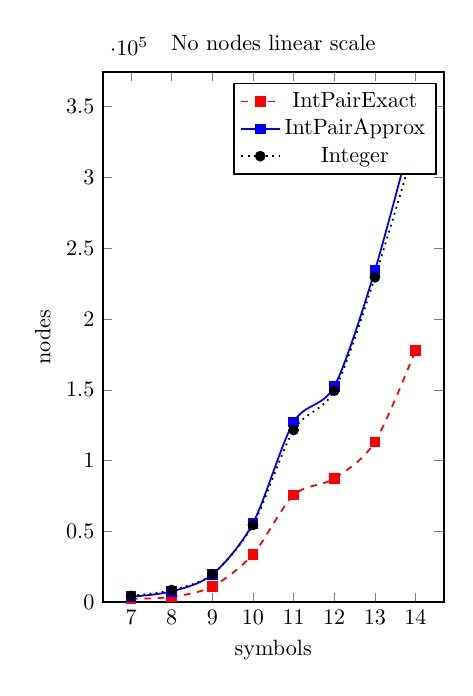
\begin{tikzpicture} [scale=0.8]
    \begin{axis}[
        title=No nodes linear scale,
        ylabel=nodes,
        xtick=data,
        ymin=0, 
        xlabel=symbols ]
      \addplot[smooth,mark=square*, mark options={solid},red, dashed]
      coordinates{ (7, 2397) (8, 3806) (9, 11079) (10, 33853) (11, 75698) (12, 87336) (13, 113148) (14, 177889)
      }; \label{ie_plot} \addlegendentry{IntPairExact}
      \addplot[smooth,mark=square*, mark options={solid},blue]
      coordinates{ (7, 3900) (8, 7665) (9, 19595) (10, 55807) (11, 127240) (12, 152406) (13, 234257) (14, 340410)
      }; \label{ia_plot} \addlegendentry{IntPairApprox}
      \addplot[smooth,mark=*,mark options={solid},black, dotted]
      coordinates{ (7, 4474) (8, 8637) (9, 19738) (10, 54608) (11, 121629) (12, 149424) (13, 229421) (14, 324263)
      }; \label{int_plot} \addlegendentry{Integer}
    \end{axis}
  \end{tikzpicture}
  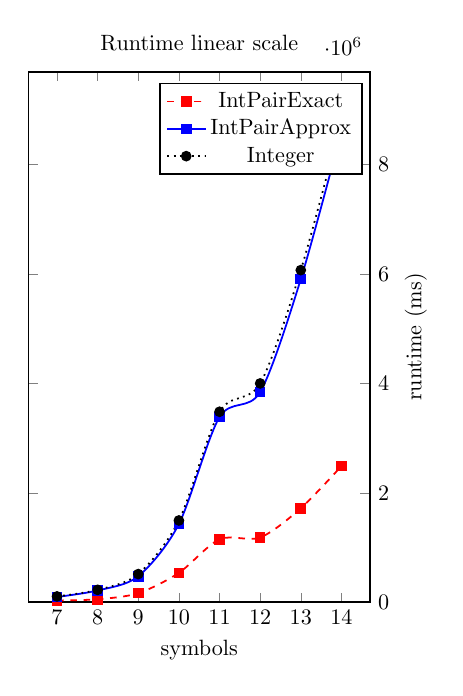
\begin{tikzpicture} [scale=0.8]
    \begin{axis}[
        yticklabel pos=right,
        xtick=data,
        title=Runtime linear scale,
        ylabel=runtime (ms),
        xlabel=symbols,
        ymin=0, ]
      \addplot[smooth,mark=square*,mark options={solid},red, dashed]
      coordinates{ (7,33465) (8,55016) (9,166184) (10,538149) (11,1151930) (12,1184668) (13,1718874) (14,2490040)
      }; \label{IntPairExact Run}
      \addplot[smooth,mark=square*,mark options={solid},blue]
      coordinates{ (7,97813) (8,215704) (9,475322) (10,1430987) (11,3386150) (12,3844124) (13,5907202) (14,8611872)
      }; \label{IntPairApprox Run}
      \addplot[smooth,mark=*,mark options={solid},black, dotted]
      coordinates{ (7,107122) (8,226900) (9,515144) (10,1495850) (11,3482780) (12,4001064) (13,6072058) (14,8813384)
      }; \label{IntegerRun}
      \addlegendentry{IntPairExact}
      \addlegendentry{IntPairApprox}
      \addlegendentry{Integer}
    \end{axis}
  \end{tikzpicture}

  
\begin{tikzpicture}[scale=1.4]
    \draw[very thick] (-4,0) -- (4,0);
    \draw[draw=white] (-5,-0.2) -- (5,-0.2);
  \end{tikzpicture}


  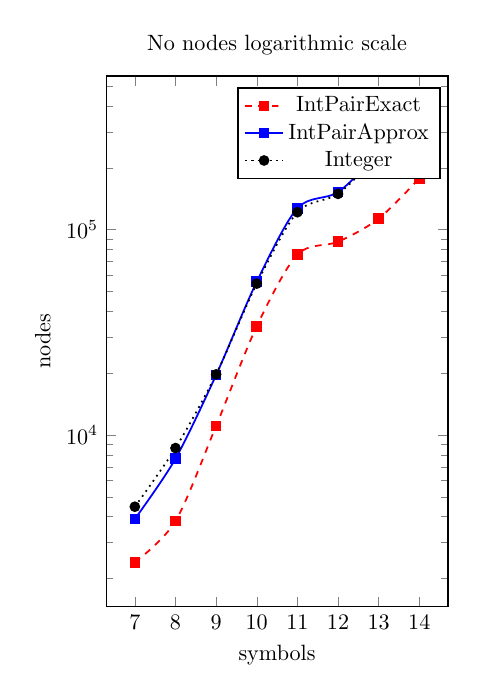
\begin{tikzpicture} [scale=0.8]
    \begin{semilogyaxis}[
        title=No nodes logarithmic scale,
        ylabel=nodes,
        xtick=data,
        ymin=0, 
        xlabel=symbols ]
     \addplot[smooth,mark=square*, mark options={solid},red, dashed]
      coordinates{ (7, 2397) (8, 3806) (9, 11079) (10, 33853) (11, 75698) (12, 87336) (13, 113148) (14, 177889)
      }; \label{ie_plot} \addlegendentry{IntPairExact}
      \addplot[smooth,mark=square*, mark options={solid},blue]
      coordinates{ (7, 3900) (8, 7665) (9, 19595) (10, 55807) (11, 127240) (12, 152406) (13, 234257) (14, 340410)
      }; \label{ia_plot} \addlegendentry{IntPairApprox}
      \addplot[smooth,mark=*,mark options={solid},black, dotted]
      coordinates{ (7, 4474) (8, 8637) (9, 19738) (10, 54608) (11, 121629) (12, 149424) (13, 229421) (14, 324263)
      }; \label{int_plot} \addlegendentry{Integer}

    \end{semilogyaxis}
  \end{tikzpicture}
  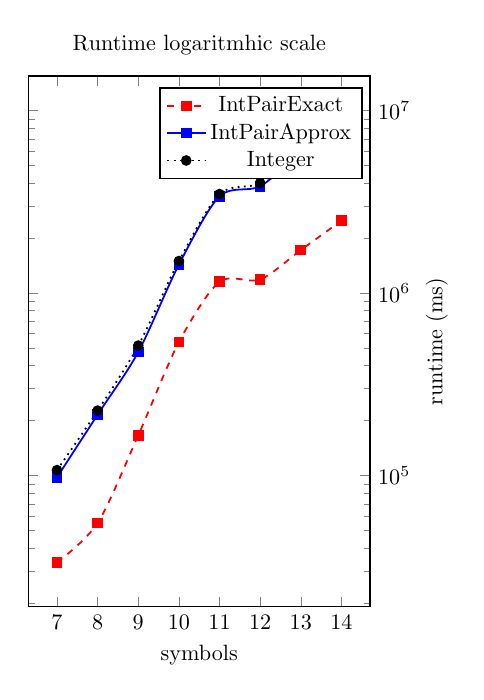
\begin{tikzpicture} [scale=0.8]
    \begin{semilogyaxis}[
        title=Runtime logaritmhic scale,
        yticklabel pos=right,
        xtick=data,
        ylabel=runtime (ms),
        xlabel=symbols,
        ymin=0,  ]
      \addplot[smooth,mark=square*,mark options={solid},red, dashed]
      coordinates{ (7,33465) (8,55016) (9,166184) (10,538149) (11,1151930) (12,1184668) (13,1718874) (14,2490040)
      }; \label{IntPairExact Run}
      \addplot[smooth,mark=square*,mark options={solid},blue]
      coordinates{ (7,97813) (8,215704) (9,475322) (10,1430987) (11,3386150) (12,3844124) (13,5907202) (14,8611872)
      }; \label{IntPairApprox Run}
      \addplot[smooth,mark=*,mark options={solid},black, dotted]
      coordinates{ (7,107122) (8,226900) (9,515144) (10,1495850) (11,3482780) (12,4001064) (13,6072058) (14,8813384)
      }; \label{IntegerRun}
      \addlegendentry{IntPairExact}
      \addlegendentry{IntPairApprox}
      \addlegendentry{Integer}
    \end{semilogyaxis}
  \end{tikzpicture}
  \caption{{Caption}}\label{fig:}
\end{figure}

\begin{figure}[H]
  \centering
  \textbf{Varying cost }
  \newline
  \newline
  \pgfplotsset{
    scale only axis,
    legend style={at={(0,0.8)}, anchor=west, font=\tiny},
    xmin=15,
  }
  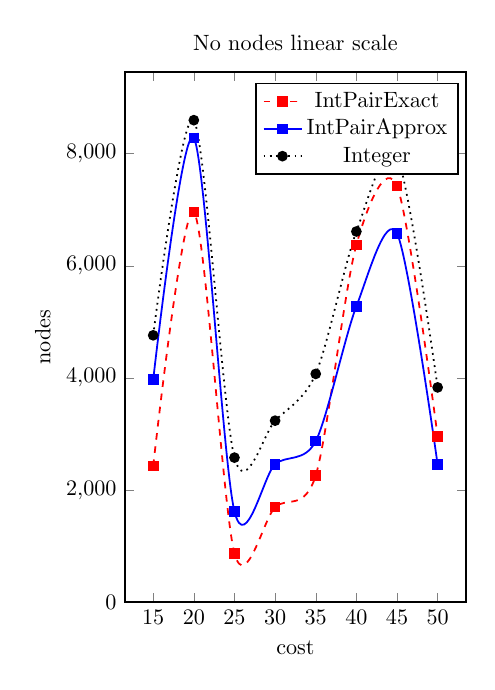
\begin{tikzpicture} [scale=0.8]
    \begin{axis}[
        title=No nodes linear scale,
        ylabel=nodes,
        xtick=data,
        ymin=0, 
        xlabel=cost ]
      \addplot[smooth,mark=square*, mark options={solid},red, dashed]
      coordinates{ (15, 2428) (20, 6960) (25, 872) (30, 1696) (35, 2261) (40, 6373) (45, 7422) (50, 2959)
      }; \label{ie_plot} \addlegendentry{IntPairExact}
      \addplot[smooth,mark=square*, mark options={solid},blue]
      coordinates{ (15, 3969) (20, 8278) (25, 1619) (30, 2461) (35, 2873) (40, 5276) (45, 6577) (50, 2455)
      }; \label{ia_plot} \addlegendentry{IntPairApprox}
      \addplot[smooth,mark=*,mark options={solid},black, dotted]
      coordinates{ (15, 4760) (20, 8596) (25, 2579) (30, 3238) (35, 4072) (40, 6611) (45, 7957) (50, 3831)
      }; \label{int_plot} \addlegendentry{Integer}
    \end{axis}
  \end{tikzpicture}
  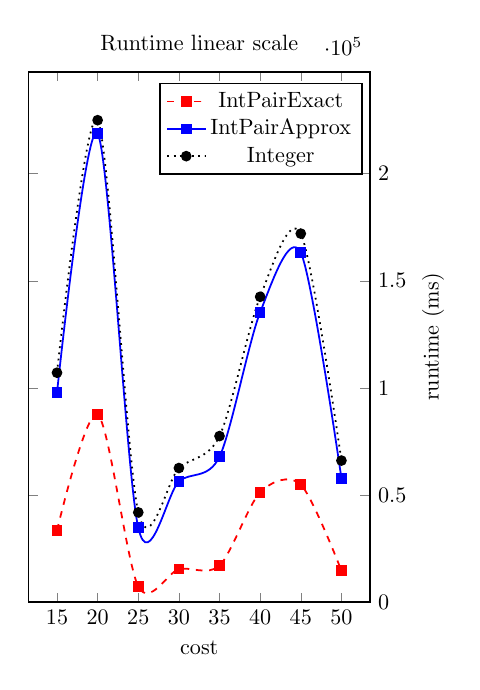
\begin{tikzpicture} [scale=0.8]
    \begin{axis}[
        yticklabel pos=right,
        xtick=data,
        title=Runtime linear scale,
        ylabel=runtime (ms),
        xlabel=cost,
        ymin=0, ]
      \addplot[smooth,mark=square*,mark options={solid},red, dashed]
      coordinates{ (15,33465) (20,87636) (25,7373) (30,15440) (35,17133) (40,51271) (45,54898) (50,14749)
      }; \label{IntPairExact Run}
      \addplot[smooth,mark=square*,mark options={solid},blue]
      coordinates{ (15,97813) (20,218750) (25,34761) (30,56398) (35,67953) (40,135341) (45,163128) (50,57833)
      }; \label{IntPairApprox Run}
      \addplot[smooth,mark=*,mark options={solid},black, dotted]
      coordinates{ (15,107122) (20,224958) (25,41936) (30,62636) (35,77550) (40,142552) (45,172028) (50,66124)
      }; \label{IntegerRun}
      \addlegendentry{IntPairExact}
      \addlegendentry{IntPairApprox}
      \addlegendentry{Integer}
    \end{axis}
  \end{tikzpicture}

  
\begin{tikzpicture}[scale=1.4]
    \draw[very thick] (-4,0) -- (4,0);
    \draw[draw=white] (-5,-0.2) -- (5,-0.2);
  \end{tikzpicture}


  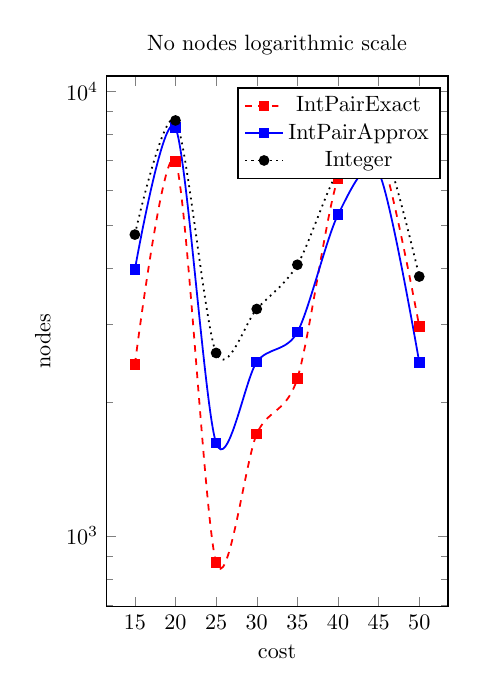
\begin{tikzpicture} [scale=0.8]
    \begin{semilogyaxis}[
        title=No nodes logarithmic scale,
        ylabel=nodes,
        xtick=data,
        ymin=0, 
        xlabel=cost ]
     \addplot[smooth,mark=square*, mark options={solid},red, dashed]
      coordinates{ (15, 2428) (20, 6960) (25, 872) (30, 1696) (35, 2261) (40, 6373) (45, 7422) (50, 2959)
      }; \label{ie_plot} \addlegendentry{IntPairExact}
      \addplot[smooth,mark=square*, mark options={solid},blue]
      coordinates{ (15, 3969) (20, 8278) (25, 1619) (30, 2461) (35, 2873) (40, 5276) (45, 6577) (50, 2455)
      }; \label{ia_plot} \addlegendentry{IntPairApprox}
      \addplot[smooth,mark=*,mark options={solid},black, dotted]
      coordinates{ (15, 4760) (20, 8596) (25, 2579) (30, 3238) (35, 4072) (40, 6611) (45, 7957) (50, 3831)
      }; \label{int_plot} \addlegendentry{Integer}

    \end{semilogyaxis}
  \end{tikzpicture}
  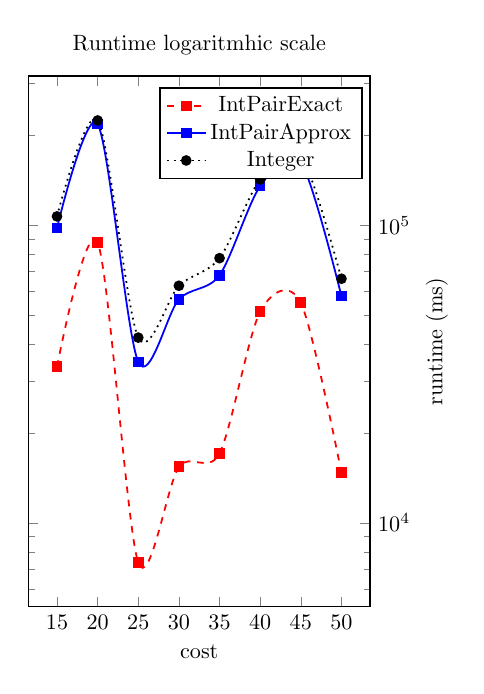
\begin{tikzpicture} [scale=0.8]
    \begin{semilogyaxis}[
        title=Runtime logaritmhic scale,
        yticklabel pos=right,
        xtick=data,
        ylabel=runtime (ms),
        xlabel=cost,
        ymin=0,  ]
      \addplot[smooth,mark=square*,mark options={solid},red, dashed]
      coordinates{ (15,33465) (20,87636) (25,7373) (30,15440) (35,17133) (40,51271) (45,54898) (50,14749)
      }; \label{IntPairExact Run}
      \addplot[smooth,mark=square*,mark options={solid},blue]
      coordinates{ (15,97813) (20,218750) (25,34761) (30,56398) (35,67953) (40,135341) (45,163128) (50,57833)
      }; \label{IntPairApprox Run}
      \addplot[smooth,mark=*,mark options={solid},black, dotted]
      coordinates{ (15,107122) (20,224958) (25,41936) (30,62636) (35,77550) (40,142552) (45,172028) (50,66124)
      }; \label{IntegerRun}
      \addlegendentry{IntPairExact}
      \addlegendentry{IntPairApprox}
      \addlegendentry{Integer}
    \end{semilogyaxis}
  \end{tikzpicture}
  \caption{{Caption}}\label{fig:}
\end{figure}

\begin{figure}[H]
  \centering
  \pgfplotsset{
    scaled y ticks=false,
    scale only axis,
    legend style={at={(0,0.8)}, anchor=west, font=\tiny},
    xmin=7,
  }
  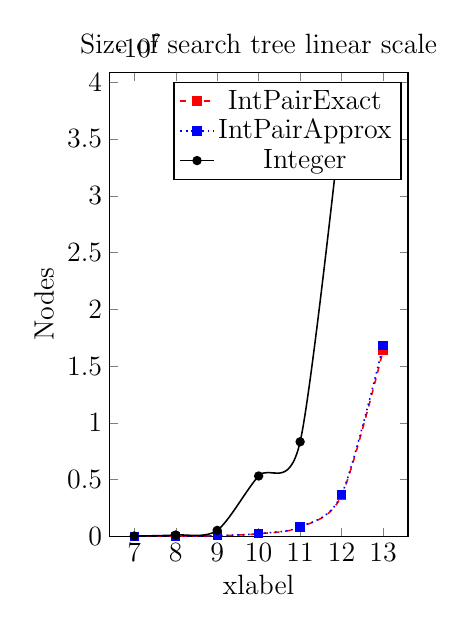
\begin{tikzpicture} [scale=0.7, font=\Large]
    \begin{axis}[
        title=Size of search tree linear scale,
        ylabel=Nodes,
        xtick=data,
        ymin=0, 
        xlabel=xlabel ]
      \addplot[smooth,mark=square*, mark options={solid},red, dashed]
      coordinates{ (7,2958) (8,12299) (9,53945) (10,233801) (11,809042) (12,3602055) (13,16361867)
      }; \label{ie_plot} \addlegendentry{IntPairExact}
      \addplot[smooth,mark=square*, mark options={solid},blue, dotted]
      coordinates{ (7,3048) (8,12623) (9,55211) (10,240131) (11,829618) (12,3696025) (13,16790307)
      }; \label{ia_plot} \addlegendentry{IntPairApprox}
      \addplot[smooth,mark=*,mark options={solid},black]
      coordinates{ (7, 28628) (8, 121116) (9, 527254) (10, 5315546) (11, 8329154) (12, 37151208)
      }; \label{int_plot} \addlegendentry{Integer}
    \end{axis}
  \end{tikzpicture}
  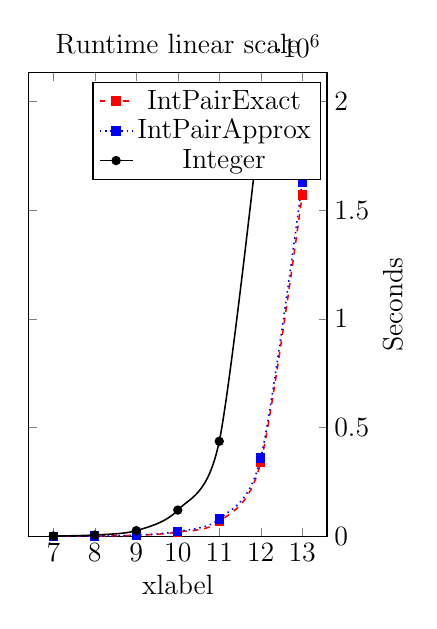
\begin{tikzpicture} [scale=0.7, font=\Large]
    \begin{axis}[
        yticklabel pos=right,
        xtick=data,
        title=Runtime linear scale,
        ylabel=Seconds,
        xlabel=xlabel,
        ymin=0, ]
      \addplot[smooth,mark=square*,mark options={solid},red, dashed]
      coordinates{ (7, 339) (8, 1142) (9, 4601) (10, 19534) (11, 67852) (12, 340757) (13, 1569780)
      }; \label{IntPairExact Run}
      \addplot[smooth,mark=square*,mark options={solid},blue, dotted]
      coordinates{ (7, 290) (8, 1263) (9, 5724) (10, 22607) (11, 80168) (12, 359915) (13, 1629885)
      }; \label{IntPairApprox Run}
      \addplot[smooth,mark=*,mark options={solid},black]
      coordinates{ (7, 1464) (8,6312) (9, 26246) (10, 120832) (11, 437171) (12, 1940096)
      }; \label{IntegerRun}
      \addlegendentry{IntPairExact}
      \addlegendentry{IntPairApprox}
      \addlegendentry{Integer}
    \end{axis}
  \end{tikzpicture}

  
\begin{tikzpicture}[scale=1.4]
    \draw[very thick] (-4,0) -- (4,0);
    \draw[draw=white] (-5,-0.2) -- (5,-0.2);
  \end{tikzpicture}


  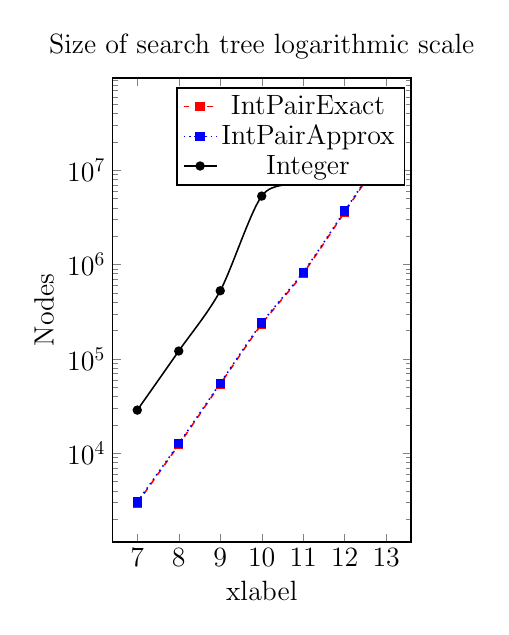
\begin{tikzpicture} [scale=0.7, font=\Large]
    \begin{semilogyaxis}[
        title=Size of search tree logarithmic scale,
        ylabel=Nodes,
        xtick=data,
        ymin=0, 
        xlabel=xlabel ]
     \addplot[smooth,mark=square*, mark options={solid},red, dashed]
      coordinates{ (7,2958) (8,12299) (9,53945) (10,233801) (11,809042) (12,3602055) (13,16361867)
      }; \label{ie_plot} \addlegendentry{IntPairExact}
      \addplot[smooth,mark=square*, mark options={solid},blue, dotted]
      coordinates{ (7,3048) (8,12623) (9,55211) (10,240131) (11,829618) (12,3696025) (13,16790307)
      }; \label{ia_plot} \addlegendentry{IntPairApprox}
      \addplot[smooth,mark=*,mark options={solid},black]
      coordinates{ (7, 28628) (8, 121116) (9, 527254) (10, 5315546) (11, 8329154) (12, 37151208)
      }; \label{int_plot} \addlegendentry{Integer}

    \end{semilogyaxis}
  \end{tikzpicture}
  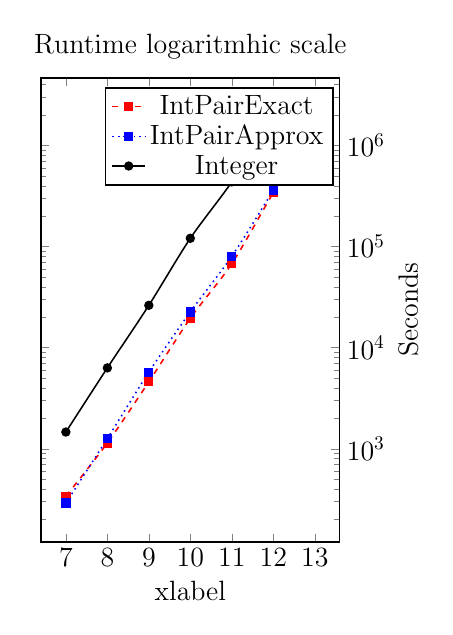
\begin{tikzpicture} [scale=0.7, font=\Large]
    \begin{semilogyaxis}[
        title=Runtime logaritmhic scale,
        yticklabel pos=right,
        xtick=data,
        ylabel=Seconds,
        xlabel=xlabel,
        ymin=0,  ]
      \addplot[smooth,mark=square*,mark options={solid},red, dashed]
      coordinates{ (7, 339) (8, 1142) (9, 4601) (10, 19534) (11, 67852) (12, 340757) (13, 1569780)
      }; \label{IntPairExact Run}
      \addplot[smooth,mark=square*,mark options={solid},blue, dotted]
      coordinates{ (7, 290) (8, 1263) (9, 5724) (10, 22607) (11, 80168) (12, 359915) (13, 1629885)
      }; \label{IntPairApprox Run}
      \addplot[smooth,mark=*,mark options={solid},black]
      coordinates{ (7, 1464) (8,6312) (9, 26246) (10, 120832) (11, 437171) (12, 1940096)
      }; \label{IntegerRun}
      \addlegendentry{IntPairExact}
      \addlegendentry{IntPairApprox}
      \addlegendentry{Integer}
    \end{semilogyaxis}
  \end{tikzpicture}
%  \input{}
%\end{figure}
  \caption{Varying the length of the string. The other parameters are fixed. Number of states=7, size of alphabet=7, and max cost per transition=15. Here we also show graphs in logarithmic scale. The integer variable timed out for $steps=13$.}\label{fig:steps}
 \end{figure}


%% symbols
\begin{figure}[H]
\centering
\textbf{Varying number of symbols}
\newline
\newline
	\pgfplotsset{
	    scale only axis,
		legend style={at={(0,0.8)}, anchor=west, font=\tiny},
	    xmin=5, xmax=8
	}
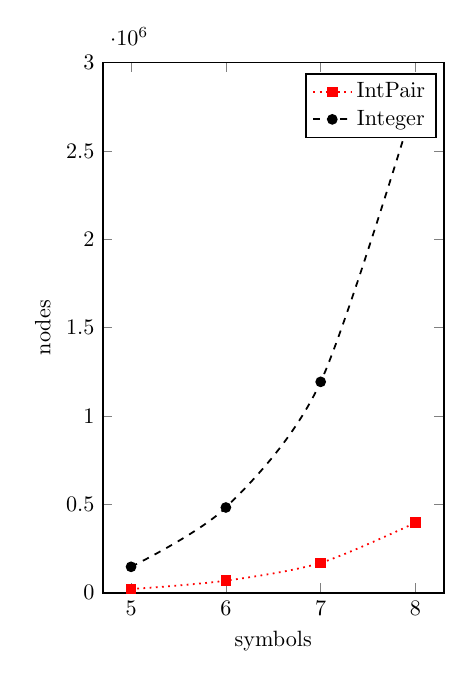
\begin{tikzpicture} [scale=0.8] 
	\begin{axis}[
	  ylabel=nodes,
	  xtick=data,
  	  ymin=0, ymax=3000000,
  	  xlabel=symbols ]
		\addplot[smooth,mark=square*, mark options={solid},red, dotted]
		  coordinates{ (5,20879) (6,68523) (7,169435) (8,396625)
		}; \label{pnt_plot} \addlegendentry{IntPair}
		\addplot[smooth,mark=*,mark options={solid},black, dashed]
		  coordinates{ (5,146895) (6,482543) (7,1193363) (8,2791621)
		}; \label{int_plot} \addlegendentry{Integer}
	\end{axis}
\end{tikzpicture}
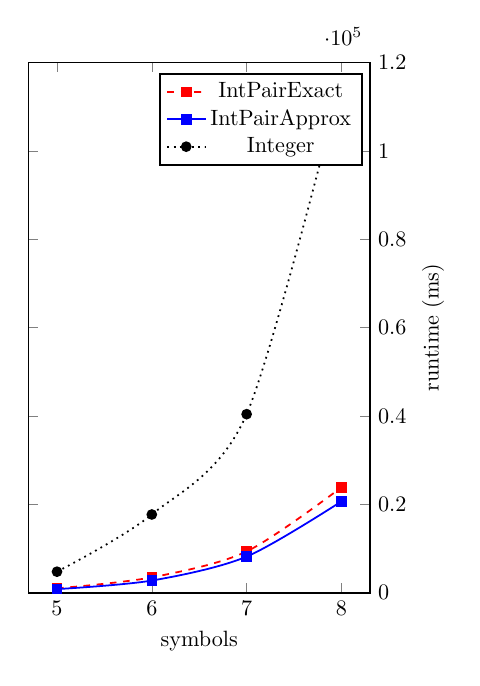
\begin{tikzpicture} [scale=0.8]
	\begin{axis}[
	yticklabel pos=right,
	  xtick=data,
	  ylabel=runtime (ms),
  	 xlabel=symbols,
	  ymin=0, ymax=120000 ] 
		\addplot[smooth,mark=square*,mark options={solid},red, dashed]
		  coordinates{ (5,992) (6,3491) (7,9352) (8,23866)
		}; \label{IntPairExact Run}
		\addplot[smooth,mark=square*,mark options={solid},blue]
		  coordinates{ (5,827) (6,2767) (7,8186) (8,20679)
		}; \label{IntPairApprox Run}
		\addplot[smooth,mark=*,mark options={solid},black, dotted]
		  coordinates{ (5,4770) (6,17716) (7,40416) (8,116126)
		}; \label{IntegerRun}
		\addlegendentry{IntPairExact}
		\addlegendentry{IntPairApprox}
		\addlegendentry{Integer}
	\end{axis}
\end{tikzpicture}
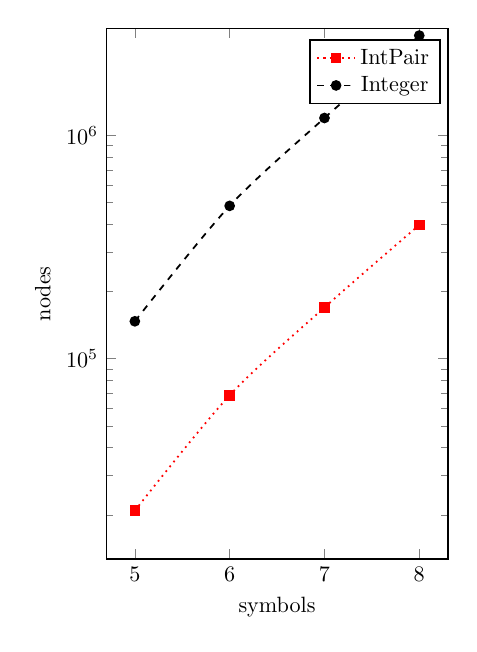
\begin{tikzpicture} [scale=0.8] 
	\begin{semilogyaxis}[
	  ylabel=nodes,
	  xtick=data,
  	  ymin=0, ymax=3000000,
  	  xlabel=symbols ]
		\addplot[smooth,mark=square*, mark options={solid},red, dotted]
		  coordinates{ (5,20879) (6,68523) (7,169435) (8,396625)
		}; \label{pnt_plot} \addlegendentry{IntPair}
		\addplot[smooth,mark=*,mark options={solid},black, dashed]
		  coordinates{ (5,146895) (6,482543) (7,1193363) (8,2791621)
		}; \label{int_plot} \addlegendentry{Integer}
	\end{semilogyaxis}
\end{tikzpicture}
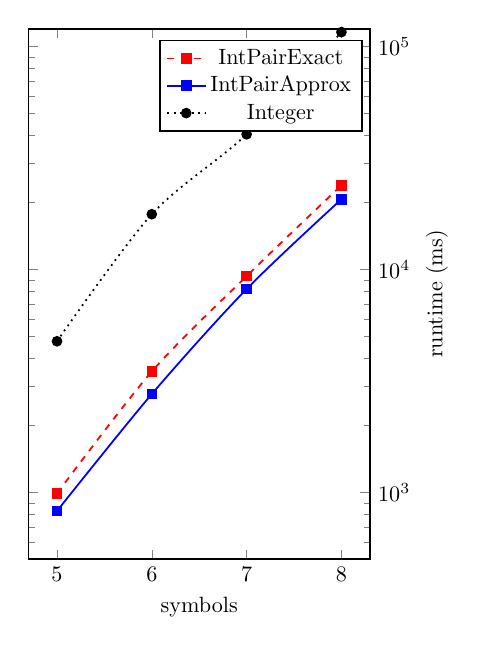
\begin{tikzpicture} [scale=0.8]
	\begin{semilogyaxis}[
	yticklabel pos=right,
	  xtick=data,
	  ylabel=runtime (ms),
  	 xlabel=symbols,
	  ymin=0, ymax=120000 ] 
		\addplot[smooth,mark=square*,mark options={solid},red, dashed]
		  coordinates{ (5,992) (6,3491) (7,9352) (8,23866)
		}; \label{IntPairExact Run}
		\addplot[smooth,mark=square*,mark options={solid},blue]
		  coordinates{ (5,827) (6,2767) (7,8186) (8,20679)
		}; \label{IntPairApprox Run}
		\addplot[smooth,mark=*,mark options={solid},black, dotted]
		  coordinates{ (5,4770) (6,17716) (7,40416) (8,116126)
		}; \label{IntegerRun}
		\addlegendentry{IntPairExact}
		\addlegendentry{IntPairApprox}
		\addlegendentry{Integer}
	\end{semilogyaxis}
\end{tikzpicture}
\caption{{States=15, Maxcost=3, Steps=6}}\label{fig:symbols}
\end{figure}


%states
\begin{figure}[H]
\centering
\textbf{Varying number of states}
\newline
\newline
	\pgfplotsset{
	    scale only axis,
		legend style={at={(0,0.4)}, anchor=west, font=\tiny},
	    xmin=20, xmax=50
	}
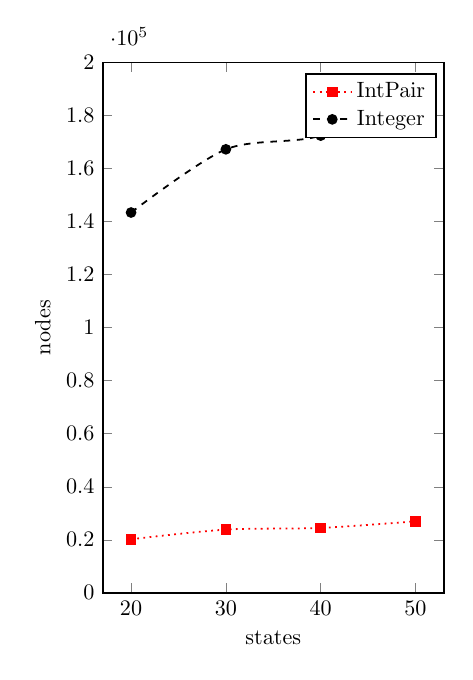
\begin{tikzpicture} [scale=0.8] 
	\begin{axis}[
	  ylabel=nodes,
	  xtick=data,
	  ymin=0, ymax=200000,
  	  xlabel=states ]
		\addplot[smooth,mark=square*, mark options={solid},red, dotted]
		  coordinates{ (20,20189) (30,23833) (40,24467) (50,26959)
		}; \label{pnt_plot} \addlegendentry{IntPair}
		\addplot[smooth,mark=*,mark options={solid},black, dashed]
		  coordinates{ (20,143413) (30,167251) (40,172417) (50,189809)
		}; \label{int_plot} \addlegendentry{Integer}
	\end{axis}
\end{tikzpicture}
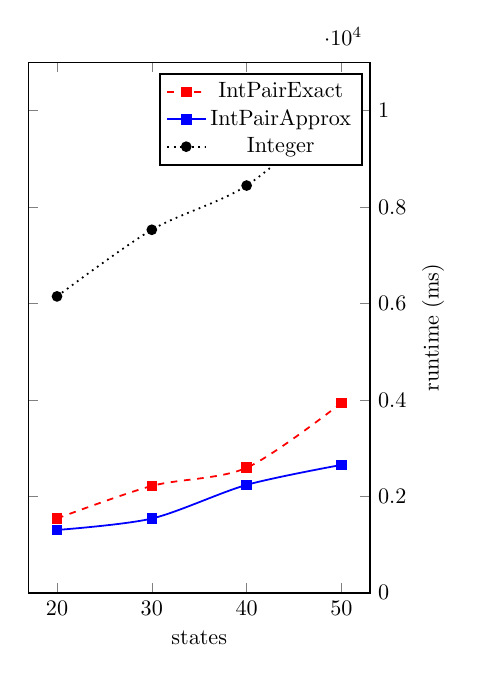
\begin{tikzpicture} [scale=0.8]
	\begin{axis}[
	yticklabel pos=right,
	  xtick=data,
	  ylabel=runtime (ms),
  	 xlabel=states,
	  ymin=0, ymax=11000 ] 
		\addplot[smooth,mark=square*,mark options={solid},red, dashed]
		  coordinates{ (20,1541)(30,2217)(40,2593) (50,3938)
		}; \label{IntPairExact Run}
		\addplot[smooth,mark=square*,mark options={solid},blue]
		  coordinates{ (20,1303) (30,1540) (40,2238) (50,2653)
		}; \label{IntPairApprox Run}
		\addplot[smooth,mark=*,mark options={solid},black, dotted]
		  coordinates{ (20,6148) (30,7530) (40,8447) (50,10086)
		}; \label{IntegerRun}
		\addlegendentry{IntPairExact}
		\addlegendentry{IntPairApprox}
		\addlegendentry{Integer}
	\end{axis}
\end{tikzpicture}
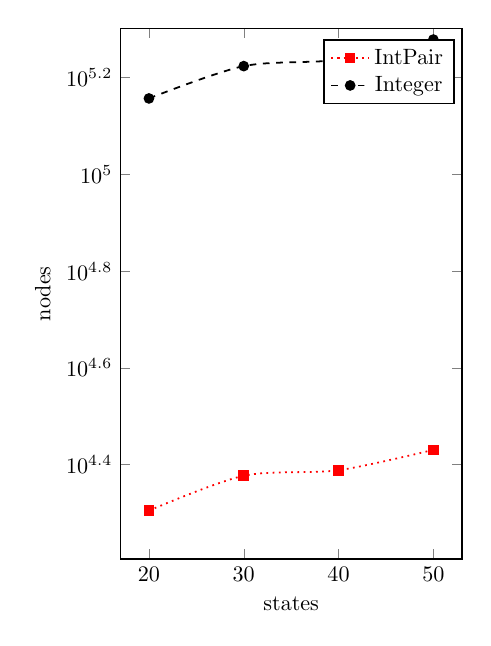
\begin{tikzpicture} [scale=0.8] 
	\begin{semilogyaxis}[
	  ylabel=nodes,
	  xtick=data,
	  ymin=0, ymax=200000,
  	  xlabel=states ]
		\addplot[smooth,mark=square*, mark options={solid},red, dotted]
		  coordinates{ (20,20189) (30,23833) (40,24467) (50,26959)
		}; \label{pnt_plot} \addlegendentry{IntPair}
		\addplot[smooth,mark=*,mark options={solid},black, dashed]
		  coordinates{ (20,143413) (30,167251) (40,172417) (50,189809)
		}; \label{int_plot} \addlegendentry{Integer}
	\end{semilogyaxis}
\end{tikzpicture}
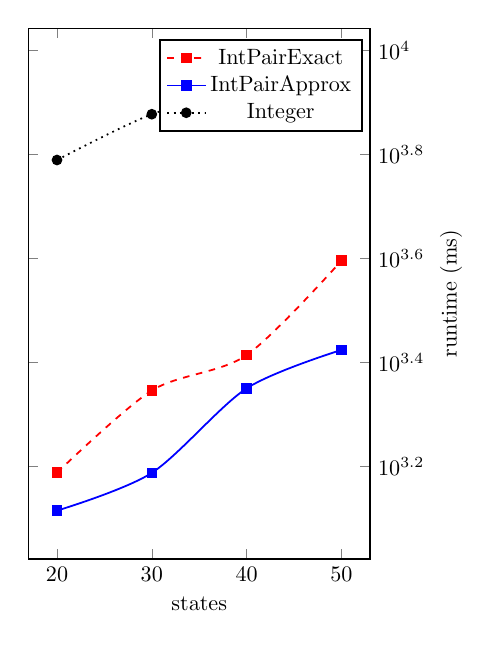
\begin{tikzpicture} [scale=0.8]
	\begin{semilogyaxis}[
	yticklabel pos=right,
	  xtick=data,
	  ylabel=runtime (ms),
  	 xlabel=states,
	  ymin=0, ymax=11000 ] 
		\addplot[smooth,mark=square*,mark options={solid},red, dashed]
		  coordinates{ (20,1541)(30,2217)(40,2593) (50,3938)
		}; \label{IntPairExact Run}
		\addplot[smooth,mark=square*,mark options={solid},blue]
		  coordinates{ (20,1303) (30,1540) (40,2238) (50,2653)
		}; \label{IntPairApprox Run}
		\addplot[smooth,mark=*,mark options={solid},black, dotted]
		  coordinates{ (20,6148) (30,7530) (40,8447) (50,10086)
		}; \label{IntegerRun}
		\addlegendentry{IntPairExact}
		\addlegendentry{IntPairApprox}
		\addlegendentry{Integer}
	\end{semilogyaxis}
\end{tikzpicture}
\caption{{Token=5, Maxcost=3, Steps=6}}\label{fig:states}
\end{figure}

%max cost
\begin{figure}[H]
\centering
\textbf{Varying maximum cost per transision}
\newline
\newline
	\pgfplotsset{
	    scale only axis,
		legend style={at={(0,0.4)}, anchor=west, font=\tiny},
	    xmin=2, xmax=15
	}
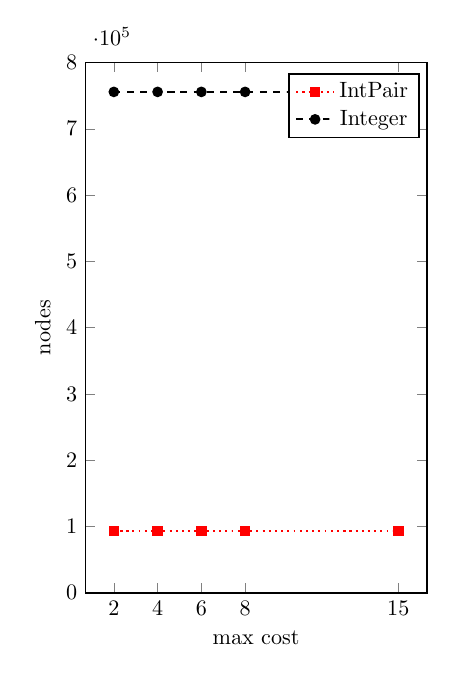
\begin{tikzpicture} [scale=0.8] 
	\begin{axis}[
	  ylabel=nodes,
	  xtick=data,
  	  ymin=2, ymax=800000,
  	  xlabel=max cost ]
		\addplot[smooth,mark=square*, mark options={solid},red, dotted]
		  coordinates{ (2,93227) (4,93227) (6,93227) (8,93227) (15,93227)
		}; \label{pnt_plot} \addlegendentry{IntPair}
		\addplot[smooth,mark=*,mark options={solid},black, dashed]
		  coordinates{ (2,755629) (4,755629) (6,755629) (8,755629) (15,755629)
		}; \label{int_plot} \addlegendentry{Integer}
	\end{axis}
\end{tikzpicture}
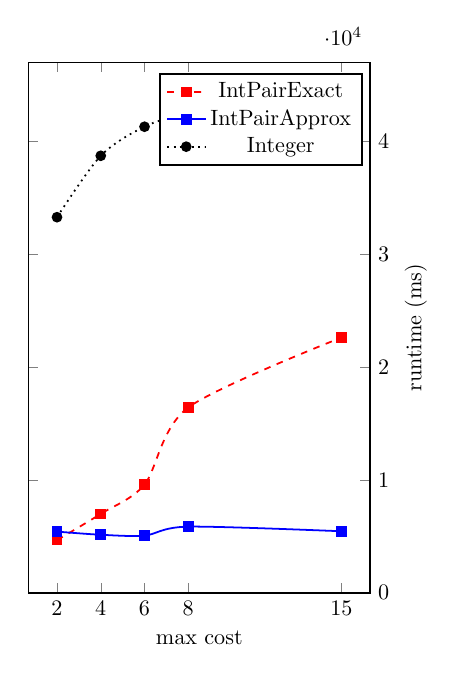
\begin{tikzpicture} [scale=0.8]
	\begin{axis}[
	yticklabel pos=right,
	  xtick=data,
	  ylabel=runtime (ms),
  	 xlabel=max cost,
	  ymin=0, ymax=47000 ] 
		\addplot[smooth,mark=square*,mark options={solid},red, dashed]
		  coordinates{ (2,4669) (4,6994) (6,9594) (8,16423) (15,22621)
		}; \label{IntPairExact Run}
		\addplot[smooth,mark=square*,mark options={solid},blue]
		  coordinates{ (2,5423) (4,5143)(6,5069) (8,5862) (15,5452)
		}; \label{IntPairApprox Run}
		\addplot[smooth,mark=*,mark options={solid},black, dotted]
		  coordinates{ (2,33288) (4,38731) (6,41307) (8,42426) (15,44868)
		}; \label{IntegerRun}
		\addlegendentry{IntPairExact}
		\addlegendentry{IntPairApprox}
		\addlegendentry{Integer}
	\end{axis}
\end{tikzpicture}
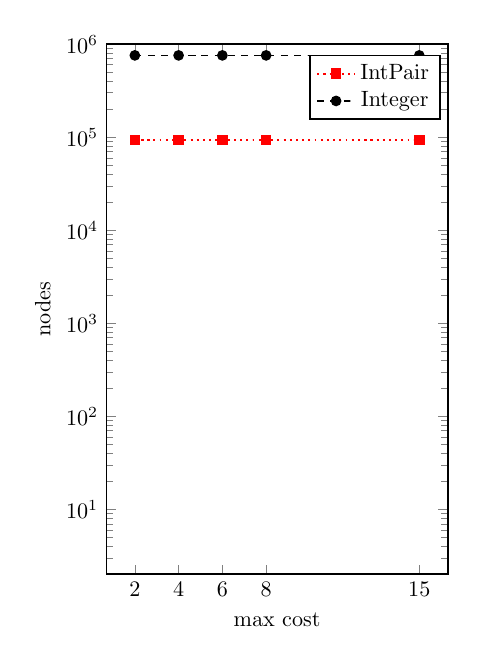
\begin{tikzpicture} [scale=0.8] 
	\begin{semilogyaxis}[
	  ylabel=nodes,
	  xtick=data,
  	  ymin=2, ymax=1000000,
  	  xlabel=max cost ]
		\addplot[smooth,mark=square*, mark options={solid},red, dotted]
		  coordinates{ (2,93227) (4,93227) (6,93227) (8,93227) (15,93227)
		}; \label{pnt_plot} \addlegendentry{IntPair}
		\addplot[smooth,mark=*,mark options={solid},black, dashed]
		  coordinates{ (2,755629) (4,755629) (6,755629) (8,755629) (15,755629)
		}; \label{int_plot} \addlegendentry{Integer}
	\end{semilogyaxis}
\end{tikzpicture}
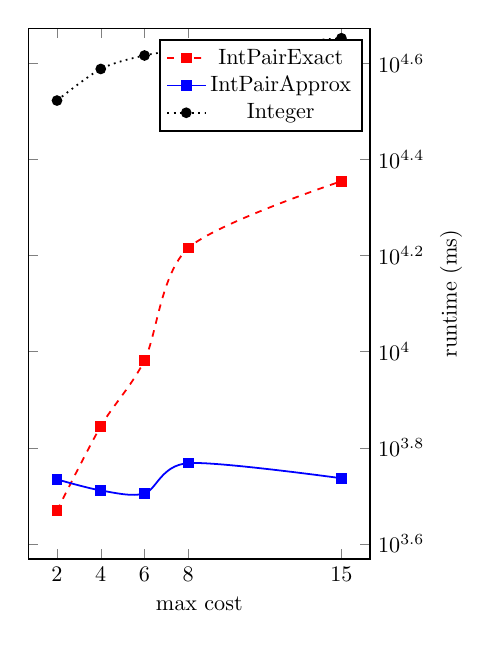
\begin{tikzpicture} [scale=0.8]
	\begin{semilogyaxis}[
	yticklabel pos=right,
	  xtick=data,
	  ylabel=runtime (ms),
  	 xlabel=max cost,
	  ymin=0, ymax=47000 ] 
		\addplot[smooth,mark=square*,mark options={solid},red, dashed]
		  coordinates{ (2,4669) (4,6994) (6,9594) (8,16423) (15,22621)
		}; \label{IntPairExact Run}
		\addplot[smooth,mark=square*,mark options={solid},blue]
		  coordinates{ (2,5423) (4,5143)(6,5069) (8,5862) (15,5452)
		}; \label{IntPairApprox Run}
		\addplot[smooth,mark=*,mark options={solid},black, dotted]
		  coordinates{ (2,33288) (4,38731) (6,41307) (8,42426) (15,44868)
		}; \label{IntegerRun}
		\addlegendentry{IntPairExact}
		\addlegendentry{IntPairApprox}
		\addlegendentry{Integer}
	\end{semilogyaxis}
\end{tikzpicture}
\caption{{Steps=20, Tokens=5, Steps=7. }}\label{fig:cost}
\end{figure}

%steps
\begin{figure}[H]
\centering
\textbf{Varying number of steps}
\newline
\newline

	\pgfplotsset{
	    scale only axis,
		legend style={at={(0,0.4)}, anchor=west, font=\tiny},
	    xmin=7, xmax=10
	}
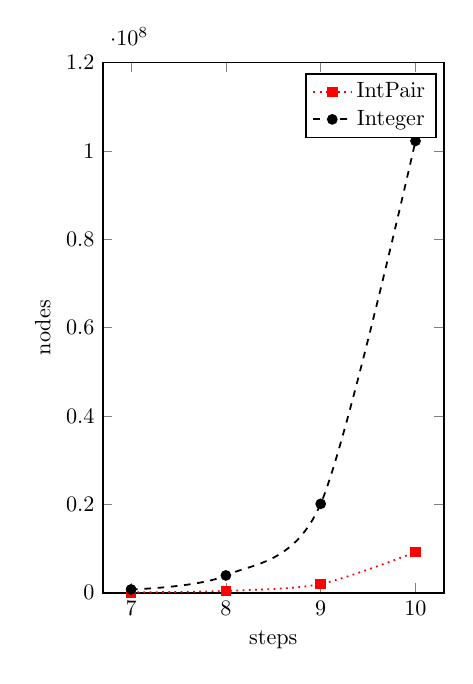
\begin{tikzpicture} [scale=0.8] 
	\begin{axis}[
	  ylabel=nodes,
	  xtick=data,
  	  ymin=2, ymax=120000000,
  	  xlabel=steps ]
		\addplot[smooth,mark=square*, mark options={solid},red, dotted]
		  coordinates{ (7,93227)  (8,431051) (9,1992011) (10,9207489)
		}; \label{pnt_plot} \addlegendentry{IntPair}
		\addplot[smooth,mark=*,mark options={solid},black, dashed]
		  coordinates{ (7,755629)(8,3924361)(9,20128261) (10,102243101)
		}; \label{int_plot} \addlegendentry{Integer}
	\end{axis}
\end{tikzpicture}
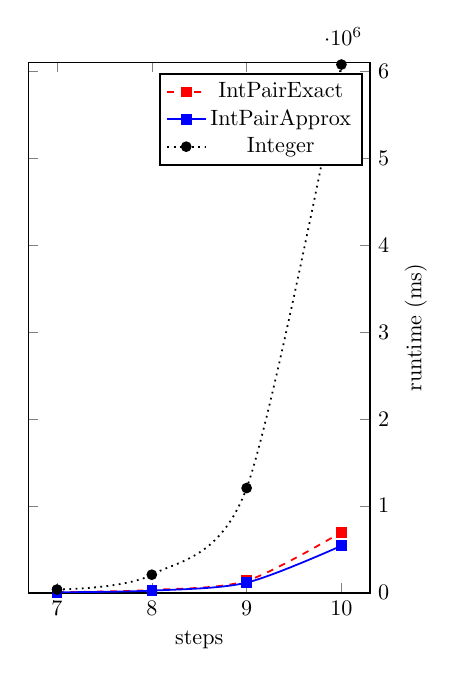
\begin{tikzpicture} [scale=0.8]
	\begin{axis}[
	yticklabel pos=right,
	  xtick=data,
	  ylabel=runtime (ms),
  	 xlabel=steps,
	  ymin=0, ymax=6100000] 
		\addplot[smooth,mark=square*,mark options={solid},red, dashed]
		  coordinates{ (7,6535) (8,32150) (9,137846) (10,696655)
		}; \label{IntPairExact Run}
		\addplot[smooth,mark=square*,mark options={solid},blue]
		  coordinates{ (7,5582)(8,24569)(9,116613) (10,540708)
		}; \label{IntPairApprox Run}
		\addplot[smooth,mark=*,mark options={solid},black, dotted]
		  coordinates{ (7,37169) (8,207591) (9,1204695)(10,6076224)
		}; \label{IntegerRun}
		\addlegendentry{IntPairExact}
		\addlegendentry{IntPairApprox}
		\addlegendentry{Integer}
	\end{axis}
\end{tikzpicture}
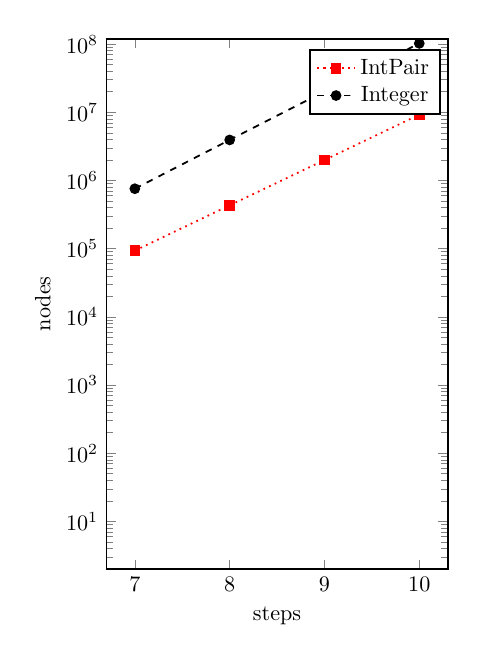
\begin{tikzpicture} [scale=0.8] 
	\begin{semilogyaxis}[
	  ylabel=nodes,
	  xtick=data,
  	  ymin=2, ymax=120000000,
  	  xlabel=steps ]
		\addplot[smooth,mark=square*, mark options={solid},red, dotted]
		  coordinates{ (7,93227)  (8,431051) (9,1992011) (10,9207489)
		}; \label{pnt_plot} \addlegendentry{IntPair}
		\addplot[smooth,mark=*,mark options={solid},black, dashed]
		  coordinates{ (7,755629)(8,3924361)(9,20128261) (10,102243101)
		}; \label{int_plot} \addlegendentry{Integer}
	\end{semilogyaxis}
\end{tikzpicture}
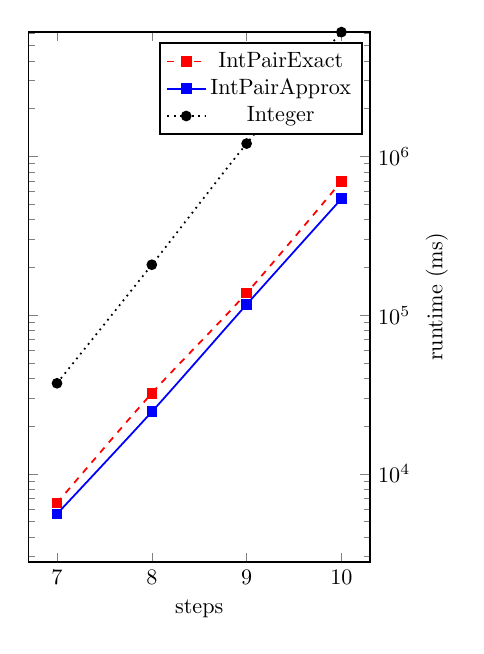
\begin{tikzpicture} [scale=0.8]
	\begin{semilogyaxis}[
	yticklabel pos=right,
	  xtick=data,
	  ylabel=runtime (ms),
  	 xlabel=steps,
	  ymin=0, ymax=6100000] 
		\addplot[smooth,mark=square*,mark options={solid},red, dashed]
		  coordinates{ (7,6535) (8,32150) (9,137846) (10,696655)
		}; \label{IntPairExact Run}
		\addplot[smooth,mark=square*,mark options={solid},blue]
		  coordinates{ (7,5582)(8,24569)(9,116613) (10,540708)
		}; \label{IntPairApprox Run}
		\addplot[smooth,mark=*,mark options={solid},black, dotted]
		  coordinates{ (7,37169) (8,207591) (9,1204695)(10,6076224)
		}; \label{IntegerRun}
		\addlegendentry{IntPairExact}
		\addlegendentry{IntPairApprox}
		\addlegendentry{Integer}
	\end{semilogyaxis}
\end{tikzpicture}
\caption{{States=20, Tokens=5, Maxcost=4}}\label{fig:steps}
\end{figure}

 


In the graphs we can see advantages for the pair variables. In all tests they are more efficient than using regular integer variables in both execution time and size of the search tree. However, it does so at the cost of higher memory usage per node. A node in the integer variable variant uses five integer variables, while the pair variants use two pair variables and one integer variable. The size of a node for the IntVar variable case should be roughly proportional to $Steps\cdot (States + Maxtotalcost)$ plus some overhead, but for the exact pair case the domain sizes of the pairs is proportional to the number of states times the max total cost. This means that the size per node is proportional to $Steps\cdot States\cdot Maxtotalcost$. With approximate pairs, the size per node is proportional to $Steps\cdot States$. For two-dimensional tuples with relatively small domain sizes, this should not be of any concern. However, higher dimensions could cause troubles. The cDFA problem could be modelled with a five-dimensional tuple variable. For a case with 50 states, 5 symbols, 6 steps and a maximum total cost of 18, the size per node would be around 100MB. Note though that the tuple variables have a higher memory usage \textit{per node} and that this does not necessarily mean that the total memory usage is higher, since the number of nodes in the search tree shrinks. The case where the memory would be a problem is if the search tree became to deep, because a parent node can not be freed from memory until its children have been propagated to either a failure or a solution.

When experiments were run (this is not shown in any graph) with the maximum total cost being bounded only from one side, the number of nodes is exactly equal for both exact pairs and approximate pairs. This confirms a conclusion from Beldiceanu et al. \cite{Beldiceanu675954}, which states that it is possible to achieve domain consistency when the cost is not restricted from both direction. In the graphs, the cost is constrained from both directions. This means that the search tree using exact pairs is \textit{at most} as large as the corresponding tree using approximate pairs. However, the differences are barely visible.

In Figure~\ref{fig:steps}, the logarithmic graphs are close to straight lines. This indicates that all algorithms are exponential in both time and size of the search tree with respect to the length of the string. Since the lines are parallel, we can also see that they have the same exponential base. More importantly, this confirms that there was no complexity difference between pair variables and integer variables when solving this particular problem. Pair variables are faster, but not necessarily asymptotically faster. 

Figure~\ref{fig:states} and~\ref{fig:cost} fluctuate very much. The difficulty of the problem does not seem to depend very much on the size of parameter. When changing the number of states, the random generator generates completely different cDFAs. Changing the number of symbols also generate different cDFAs, but not in such a high degree. In the experiments, there are ten random cDFAs for each measure point. Increasing this would probably smoothen out the curve. The reason why the graphs for varying the cost per transition fluctuates so much is different. The maximum total cost is set to the maximum cost per transition times number of steps divided by 5 and the miminum cost for the final stage depend on maximum cost, so there are actually three parameters along the x-axis. One way to solve this would be to fix the maximum total cost to a fixed value. However, this is not a good solution, because a low value would make the problem easier when the cost per transition grows. On the other hand, a high value would make the problem too easy. This does not matter so much, since all the curves have the same shape, which means that if a cDFA was hard to solve, it was hard for all three methods, making the comparison fair. In Figure~\ref{fig:cost} we can also see that the runtime graphs for exact pairs are much higher than tan the graphs for approximate pairs. This is expected, because the approximate version is more suitable for removing ranges of values.

All in all, the graphs indicate that pair variables can give a better performance for certain problems. The only possible source of error with this experiment that I can think of is that the reference propagator may not be optimised enough, but I find that highly unlikely. After all, the implementation of the integer variable shipped with Gecode has to be assumed to be very optimised, and the reference propagator is much more optimised than the ones for pairs.

\section{Related Work}
Beldiceanu et al. \cite{Beldiceanu675954} describe a propagator for a counter-DFA. It is defined as a regular DFA with only accepting states and such that the transition function not only returns the next state, but the increase for a counter. The cDFA used in this thesis are almost identical. The main difference is that we also use non-accepting states. The other difference is more philosophical. Instead of counting, we talk about cost, but it makes no difference in practice. Doing a performance comparison with their implementation would be complicated to do, because their propagators are implemented in Prolog, while everything in this thesis is implemented in C++.

Kellen Dye has implemented a bitvector variable for Gecode for his master thesis \cite{Dye761927}. His report was useful for getting more understanding of how to implement a new variable in Gecode.

Monette et al.\cite{Monette771427} show that tuple variables can be used to make pruning much more efficient. This thesis is a practical demonstration of their results, and that it translates into better performance.

\section{Conclusions and future work}
The experiments show that tuple variables have potential. Both versions perform better than the integer variable variant on a cDFA problem, in both number of nodes and total execution time, and there is still much room for further improvement. Especially the vector operations are very inefficient and can easily be improved. Using the pair variable improved the speed by around \SI{700}{\percent} in these experiments. The improvement of the size of the search tree was similar.

All large software libraries have coding standards. There is plenty of work to rewrite the code for pairs in such a way that it satisfies Gecode standards. For instance, vectors from the standard library are not allowed. Furthermore, the code is far from ready in other aspects. It contains only the methods needed to run the tests in this thesis. One example of this is that it exists methods to get the minimum and maximum value for the first dimension, but no methods for the second. Also, the propagators currently only accepts arrays. 

In this thesis, there is one exact and one approximate version. The approximation is exact in one dimension and only stores the boundaries for the second. This is just one way of doing it and there are several other ways of approximating the domain. Another relevant change that could be made is to extend the pairs to arbitrary dimensions. A tuple of higher dimension would make it possible to shrink the search tree for a cDFA problem even further.

\bibliographystyle{plain}
\bibliography{bib}
%\printbibliography

%\begin{btSect}[plain]{bibliography}
%\section*{References}
% \btPrintAll
%\end{btSect}

%\begin{thebibliography}{9}
%\bibitem{propreg}
%  Beldiceanu, Flener, Pearson, Van Hentenryck,
%  \emph{Propagating Regular Counting Constraints},
%
%\bibitem{bitvector}
%  Dye,
%  \emph{Implementation of bit-vector variables in a CP solver},
%
%\bibitem{propframe}
%  Monette, Flener, Pearson,
%  \emph{A propagator design framework for constraints over sequences},
%
%\bibitem{mpg}
%  Schulte, Tack, Lagerkvist
%  \emph{Modeling and Programming with Gecode},
%
%\end{thebibliography}
\end{document}
